\documentclass[12pt]{article}
\usepackage{graphicx,psfrag,float,mathbbol,xcolor,cleveref}
\usepackage{arydshln}
\usepackage{amsfonts}
\usepackage{amsmath}
\usepackage{tikz}
\usepackage[mathscr]{euscript}
\usepackage[utf8]{inputenc}
\usepackage[english]{babel}
\usepackage{natbib} 
\usepackage[T1]{fontenc}
\usepackage{enumitem}
\usepackage{accents}
\usepackage{framed}
\usepackage{subcaption}
\usepackage{mathtools}
\usepackage{IEEEtrantools}
\usepackage{times}
\usepackage{amsthm}
\usepackage{tabularx,ragged2e,booktabs,caption}


\newcolumntype{C}[1]{>{\Centering}m{#1}}
\renewcommand\tabularxcolumn[1]{C{#1}}
\usepackage[letterpaper, left=1in, top=1in, right=1in, bottom=1in,nohead,includefoot, verbose, ignoremp]{geometry}
\newcommand{\comment}[1]{\text{\phantom{(#1)}} \tag{#1}}
\newcommand{\ms}{\scriptscriptstyle}
\newcommand\numberthis{\addtocounter{equation}{1}\tag{\theequation}}
\newcommand*\needsparaphrased{\color{red}}
\newcommand*\needscited{\color{orange}}
\newcommand*\needsproof{\color{blue}}
\newcommand*\outlineskeleton{\color{green}}
\newcommand{\PP}{\mathcal{P}}
\newcommand{\R}{\mathbb{R}}
\newcommand{\bfeps}{\mbox{\boldmath $\epsilon$}}
\newcommand{\bfgamma}{\mbox{\boldmath $\gamma$}}
\newcommand{\bflam}{\mbox{\boldmath $\lambda$}}
\newcommand{\bfphi}{\mbox{\boldmath $\phi$}}
\newcommand{\bfsigma}{\mbox{\boldmath $\sigma$}}
\newcommand{\bfbeta}{\mbox{\boldmath $\beta$}}
\newcommand{\bfalpha}{\mbox{\boldmath $\alpha$}}
\newcommand{\bfe}{\mbox{\boldmath $e$}}
\newcommand{\bff}{\mbox{\boldmath $f$}}
\newcommand{\bfone}{\mbox{\boldmath $1$}}
\newcommand{\bft}{\mbox{\boldmath $t$}}
\newcommand{\bfo}{\mbox{\boldmath $0$}}
\newcommand{\bfO}{\mbox{\boldmath $O$}}
\newcommand{\bfx}{\mbox{\boldmath $x$}}
\newcommand{\bfX}{\mbox{\boldmath $X$}}
\newcommand{\bfz}{\mbox{\boldmath $z$}}


\newcommand{\bfm}{\mbox{\boldmath $m}}
\newcommand{\bfy}{\mbox{\boldmath $y$}}
\newcommand{\bfa}{\mbox{\boldmath $a$}}
\newcommand{\bfb}{\mbox{\boldmath $b$}}
\newcommand{\bfY}{\mbox{\boldmath $Y$}}
\newcommand{\bfS}{\mbox{\boldmath $S$}}
\newcommand{\bfZ}{\mbox{\boldmath $Z$}}
\newcommand{\cardT}{\vert \mathcal{T} \vert}

\newtheorem{theorem}{Theorem}[section]
\newtheorem{lemma}[theorem]{Lemma}
\newtheorem{proposition}[theorem]{Proposition}
\newtheorem{corollary}[theorem]{Corollary}

\theoremstyle{definition}
\newtheorem{definition}{Definition}[section]
\newtheorem{example}{Example}[section]
\def\bL{\mathbf{L}}


\makeatletter
\renewcommand{\theenumi}{\Roman{enumi}}
\renewcommand{\labelenumi}{\theenumi.}
\renewcommand{\theenumii}{\Alph{enumii}}
\renewcommand{\labelenumii}{\theenumii.}
\renewcommand{\p@enumii}{\theenumi.}
\makeatother

\bibliographystyle{abbrvnat}


\begin{document}


\title{ Nonparametric Covariance Estimation for Longitudinal Data via Penalized Tensor Product Splines}

\author{Tayler A. Blake\thanks{The Ohio State University, 1958 Neil Avenue, Columbus, OH 43201} \and  Yoonkyung Lee\thanks{The Ohio State University, 1958 Neil Avenue, Columbus, OH 43201}}

\maketitle

\begin{abstract}
With high dimensional longitudinal and functional data becoming much more common, there is a strong need for methods of estimating large covariance matrices. Estimation is made difficult  by the instability of sample covariance matrices in high dimensions and a positive-definite constraint we desire to impose on estimates. A Cholesky decomposition of the covariance matrix allows for parameter estimation via unconstrained optimization as well as a statistically meaningful interpretation of the parameter estimates. Regularization improves stability of covariance estimates in high dimensions, as well as in the case where functional data are sparse and individual curves are sampled at different and possibly unequally spaced time points. By viewing the entries of the covariance matrix as the evaluation of a continuous bivariate function at the pairs of observed time points, we treat covariance estimation as bivariate smoothing. 

Within regularization framework, we propose novel covariance penalties which are designed to yield natural null models presented in the literature for stationarity or short-term dependence. These penalties are expressed in terms of variation in continuous time lag and its orthogonal complement. We present numerical results and data analysis to illustrate the utility of the proposed method. \\
\\
%\begin{keywords}
{\bf keywords:} non-parametric, covariance, longitudinal data, functional data, splines, reproducing kernel Hilbert space
%\end{keywords}
\end{abstract}

\section{Introduction}

Covariance estimation with high dimensional data has has recently gained growing interest; it is generally recognized that there are two primary hurdles responsible for the difficulty in covariance estimation: the instability of sample covariance matrices in high dimensions and a positive-definite constraint we wish estimates to obey. Estimation of population covariance matrices from samples of multivariate data has been important for methods in classical multivariate data analysis, time series analysis, spatial statistics and, more recently, the growing field of statistical learning. Covariance estimates play a critical role in establishing independence or conditional independence through graphical models, constructing discriminant functions as in linear discriminant analysis (LDA) and quadratic discriminant analysis (QDA) for the classification of Gaussian data, building confidence intervals for component means and contrasts, and constructing a low-dimensional representation of data via principal components analysis (PCA). One may note that the last two techniques require an estimate of the covariance matrix, and the first two require estimation of the inverse.

Prevalent technological advances in industry and many areas of science make high dimensional longitudinal and functional data a common occurrence, arising in numerous areas including medicine, public health, biology, and environmental science with specific applications including fMRI, spectroscopic imaging, gene microarrays among many others, presenting a need for effective covariance estimation in the challenging situation where parameter dimensionality is possibly much larger than the number of observations. Additional difficulty due to constraints required to yield positive definite estimates make covariance estimation a potentially complex optimization problem. Further, most existing approaches to covariance estimation require data to be sampled at regular grid (time) points, with subjects sharing a set of common observation points. However, in many practical situations, data are irregularly sampled, and subjects may share few common observation times, and methods are needed to accommodate for data collected in this way.  

To address the challenge of enforcing positive definiteness, several have considered modeling various matrix decompositions including variance-correlation decomposition, spectral decomposition, and Cholesky decomposition. The Cholesky decomposition has received particular attention, as it which allows for a statistically meaningful interpretation as well as an unconstrained parameterization of elements of the covariance matrix. This parameterization allows for estimation to be accomplished as simply as in least squares regression. 



It is well known that the sample covariance matrix is unstable in high dimensions, and there is an extensive existing body of work addressing the issue of high dimensionality in the context of covariance estimation. See \citet{pourahmadi2011covariance} for a survey of approaches to covariance estimation from the generalized linear modeling and regularization perspectives. However, much of this work addresses high dimensionality arising from functional or times series data sampled on a dense, regular grid. With such data, it is typical that the number of time points is larger than the number of observations. Few have addressed the challenges posed by sparse longitudinal data where measurement times may be almost unique yet sparsely distributed within the observed time range for each individual in the study. In this case, high dimensionality may not be a consequence of having more measurements per subject than the number of subjects themselves, but rather because when pooled across subjects, the total number of unique observed time points is greater than the number of individuals. Incomplete and unbalanced data arise when measurement schedules with targeted time points which are not necessarily equally spaced or if there is missing data. Sparse longitudinal data arise when the measurement schedule has arbitrary or almost unique time points for every individual. A given time point may have very few individuals with corresponding measurements. 

We sidestep both issues of high dimensionality and irregularly sampled data by viewing the response as a stochastic process having continuous covariance function. Recent work outlines the use of function estimation for smoothing elements of the covariance matrix, including \citet{wu2003nonparametric},\citet{huang2007estimation}. To our knowledge, however, no previous work has applied  smoothing to both dimensions of the Cholesky factor;  we model the generalized autoregressive parameters using tensor product splines. Viewing covariance modeling as bivariate function estimation both accommodates irregularly sampled curved and permits interpolation and extrapolation of the covariance function between two measurements at any pair of time points within the time interval of interest rather than at observed pairs of time points only. The Cholesky decomposition enables covariance estimation through the estimation of a varying coefficient model. A transformation of the design point axes allows for an ANOVA-like decomposition of the coefficient function into two components, corresponding to the lag between time points and an additive component. Through this general framework, we can easily impose penalties on fitted functions to yield natural null models presented in the literature. 

\section{Cholesky Decomposition of $\Sigma$}

To present a comprehensive overview our estimation procedure, we begin with the representation of the inverse covariance matrix, $\Omega = \Sigma^{-1}$, in terms of its Cholesky decomposition (see \citet{pourahmadi2007cholesky} for a detailed discussion.) In the section to follow, we will demonstrate that this parameterization of the precision matrix is particularly attractive due to both the computational advantages as well as the convenient modeling interpretation it permits. For any positive definite matrix $\Sigma$, there exists a unique unit lower triangular matrix $T$ with diagonal entries equal to $1$ which diagonalizes $\Sigma$:

\begin{equation}
\nonumber T \Sigma T^T = D
\end{equation}
\noindent

If we assume that the data having covariance matrix $\Sigma$ follow an autoregressive model, then the entries of the Cholesky factor $T$ and $D$ enjoy a useful interpretation. Let $Y = \left( Y_{1}, Y_{2}, \dots, Y_{m} \right)^T$ be defined on a probability space with some probability measure $\mathcal{P}$ corresponding to the multivariate Normal distribution with mean $0$ and covariance $\Sigma$, and let $Y_1,Y_2,\dots, Y_m$ have associated measurement times 

\[
t_{1} < t_{2} < \dots< t_{m}.
\]


Let $\hat{y}_t$ denote the linear least-squares predictor of $y_t$ based on its predecessors $y_1,\dots, y_{t-1}$, and let $e_t$ denote its prediction error with variance $Var\left(e_t\right)=\sigma_t^2$, $Cov\left(e_i,e_j\right)=0$ for $i \ne j$. Standard regression theory gives us that we can find coefficients $\phi_{tj}$ such that

\begin{equation}
{y}_{j}  = \sum_{k=1}^{j-1} \phi_{jk} y_{k} + \sigma_{j}e_{j}, \qquad j=2,\dots,m, \label{eq:ARmodel}.
\end{equation}

 Let $T$ denote the $m \times m$  matrix with elements 

\[
T_{jk} = \left\{
\begin{array}{ll}
-\phi_{jk} & j > k\\
1 & j = k \\
0 & otherwise,
\end{array}\right.
\]
\noindent
for $j,k=1,\dots,m$. Then in matrix notation,  model~\ref{eq:ARmodel} may then be written

\begin{equation}
e = T Y, \label{eq:epsilon}
\end{equation}
\noindent

Taking covariances on both sides of \ref{eq:epsilon}, we have

\begin{equation} \label{eq:cholesky_decomp}
D = T \Sigma T^T 
\end{equation} 

An attractive feature of this reparameterisation is that, regardless of the modelling approach, the estimated covariance matrix is guaranteed to be positive definite. The unconstrained regression coefficients $\lbrace \phi_{jk} \rbrace$ are referred to as the \emph{generalized autoregressive parameters} (GARPs). The $\lbrace \sigma^2_{j} \rbrace$ are called the \emph{innovation variances} (IVs.)  Unconstrained estimation of the $\left\{ \sigma_{k}^2 \right\}$ is achieved by log transformation;  we leave these details for section 2. Expressing the precision matrix  in terms of the GARPs and IVs, we have
\begin{equation} \label{eq:omega_decomp}
\Omega= \Sigma^{-1} = T^T D^{-1} T.
\end{equation}

Rather than estimating a specific covariance matrix for data observed on a fixed, regular grid, we aim to estimate a smooth covariance function. This accomodates data which may consist of  observations on multiple subjects measured at potentially unequally spaced and individual-specific times. In estimation of the means $\mu$ of p-vectors of i.i.d. variables, the
Gaussian white noise model [9] is the appropriate infinite-dimensional model into
which all objects of interest are embedded. In estimation of matrices, a natural
analogue is the space B(l2,l2), which we write as B, of bounded linear operators
from l2 to l2. These can be represented as matrices [cite \textit{Regularized estimation of large covariance matrices by Bickel and Levina - section 4.}]

Rather than $m$-dimensional vectors, consider $Y$ and $e$ as the values of the stochastic processes $Y\left(t\right)$ and $e\left(t\right)$ at the set of observation times.  We assume that $Y\left(t\right)$ is equipped with covariance function $G\left(s,t\right)$, and
\[
e\left(s\right) \sim \mathcal{WN}\left(0,1\right)
\] 
is a zero mean Gaussian white noise process with unit variance. We assume that $G\left(s,t\right)$ satisfies some smoothness conditions, where smoothness is defined in terms of square integrability of certain derivatives. [TODO: clean up statement about smoothness of covariance function; integrability of covariance function of a stochastic process?] The entries of $\Sigma$, then, correspond to $G$ evaluated at the distinct pairs of observed time points. Similarly, we treat the elements of the precision matrix $\Omega$ as the values of some smooth function, $\omega\left(s,t\right)$ evaluated at observed pairs of time points.


Extending this perspective to the elements of $D$ and the elements of the Cholesky factor $T$ leads us to  %view the GARPs $\lbrace \phi_{ijk} \rbrace$ and innovation variances as the evaluation of the smooth functions $\phi\left(s,t\right)$ and $\sigma^2\left(t\right)$ at observed time points and interpret $\phi_{ijk} = \phi\left(t_{ij},t_{ik}\right)$ and $\sigma_{ij}^2 = \sigma^2\left(t_{ij}\right)$. 
the varying coefficient (VC) models first introduced by Hastie and Tibshirani. 
The procedures presented by \citet{fan2000two} and \citet{huang2002varying} utilize varying coefficient models for modeling the mean of longitudinal data; parameterizing the covariance matrix according to \ref{eq:cholesky_decomp} allows us to exploit these models in covariance estimation for such data as well.  A generalization of traditional linear regression models, varying coefficient models offer more flexibility than their static analogues by allowing the effect of covariates to change smoothly with the value other variables. Both regressors and response variables are assumed to vary according to an \emph{indexing variable}, which is particularly attractive because this permits interpolation of regressors and response variables at values of this indexing variable where there is either missing data of only a single observation and slope estimation is not feasible.  Replacing  $\left \{ \phi_{jk} \right\}$ and $\left\{ \sigma_j \right\}$ with smooth functions, we model 

\begin{equation}   
y\left(t_j \right)  = \sum_{k=1}^{j-1} \phi\left(t_j ,t_k\right) y\left(t_k\right) + \sigma\left(t_j\right)\epsilon\left({t_j}\right) \;\;\;\; j=1,\dots, m, 
\label{eq:MyModel} 
\end{equation}

\noindent for $t_1 < t_2 < \dots < t_m$. 

We represent the varying coefficient function and the innovation variances using tensor product smoothing splines and penalized tensor product B-splines alongside penalties to induce simplicity in $\phi$ and $\sigma^2$  to produce final covariance estimates exhibiting the desired null structure.  For ease of exposition, we first focus our attention on the estimation of $\phi$ assume that $\sigma^2\left(t\right)$ is fixed and known; we will later propose an iterative procedure for simultaneous estimation of $\sigma^2$ and $\phi$.    %square integrability of certain derivatives. 
Recasting the problem as the estimation of model~\ref{eq:MyModel} allows us access to the existing set of tools developed in the bivariate smoothing literature; our approach provides a flexible, comprehensive framework for covariance estimation.


\section{Penalized Maximum Likelihood Estimation of $\phi$}

We employ maximum likelihood  for the estimation of  the varying coefficient function $\phi\left(t,s\right)$ and the innovation variance function $\sigma\left(t\right)$, though neither the derivation the form of model~\ref{eq:ARmodel} nor model~\ref{eq:MyModel} via the Cholesky decomposition rely on any assumptions about the distribution of $Y$. Fixing $\sigma_j^2$,  for a sample of $N$  i.i.d. observations $Y_1,Y_2,\dots,Y_N$ from a multivariate Gaussian distribution, the negative log-likelihood as a function of $\phi_{jk}$ corresponds to the usual error sums of squares and is proportional to

\begin{equation}
-2 L\left(y_1, y_2, \dots,y_N ,\Phi \right) \propto \sum_{i=1}^N \sum_{j=2}^{m_i} \sigma\left({t_j}\right)^{-2} \left(y_{ij} - \sum_{k=1}^{j-1}\phi\left({t_{ij},t_{ik}}\right)y_{ik} \right)^2 \label{loglikelihood}
\end{equation}
\noindent
where 
\[
y_i = \left( y_{i1}, y_{i2}, \dots, y_{i,m_i}\right), \quad i=1,\dots,N 
\] 

%% explain here that we omit y_{i1} from the likelihood here because in the first stage of estimation (for $\phi$), the first observation in each vector doesn't contribute to the likelihood
\noindent
denotes the vector of observations for subject $i$ with corresponding measurement times 
\[
t_{i1} < t_{i2} < \dots < t_{i,m_i}.
\]
The form of the likelihood of $y_1,\dots,y_N$ indicates that we allow both the number of measurements as well as the observation times to varying across subjects. The $\left\{t_{ij} \right\}$ need not be evenly-spaced within or across individuals.  

In the case that subjects share a common set of observation times $t_1 < \dots < t_m$,  it is well known that the MLE for $\Sigma$, $S = \sum_{i=1}^N y_i y_i^T$ is highly unstable in high dimensions, a condition that is potentially worsened when one or more subjects has at least one observation time that is unique from the set of observation times common across subjects. To mitigate instability due to high dimensionality and simultaneously permit the estimation of $\phi\left(\cdot,\cdot\right)$ as a smooth bivariate function, we obtain a covariance estimator by applying bivariate smoothing of the elements of the Cholesky factor. 


\section{Smoothing spline representation of $\phi$}

To impose structure on the estimated varying coefficient function, we augment the negative log-likelihood \ref{eq:loglikelihood} with penalty functional, which discourages the flexibility of the fitted function. We take the estimator of $\phi$ to minimize

%\begin{itemize}
%\item {\bf Step 1:} Select $\hat{\lambda}_1$, where
\begin{equation} 
 -2 L + \lambda J_{\phi}\left(\phi\right)  \label{eq:phi-objective-fnc}.
\end{equation}
%\item {\bf Step 2:} Define $\hat{\phi}$ to the the minimizer of 

The first term in \ref{eq:phi-objective-fnc} discourages the lack of fit of $\phi$ to the data, and $\lambda$ is a smoothing parameter which controls the tradeoff between the lack of fit and amount of regularization imposed on the fitted function through the penalty, $J_\phi$. Since $\phi$ explicitly defines an inverse covariance function, imposing specific types of structure on $\phi$ is of particular interest; covariance models for longitudinal or time series data are commonly defined in terms of lag, or in the continuous case, the difference between two measurement times.  By transforming the $s-t$ input axis, we reparameterize $\phi$ and express the coefficient function in terms of   
\begin{align*}
l &= s-t \\
m &= \frac{1}{2}\left(s+t\right).
\end{align*}
\noindent
Writing $\phi$ in terms of the rotation gives the reparameterized coefficient function 
\begin{equation} \label{eq:phi-star}
\phi^*\left(l,m\right) = \phi^*\left(s-t, \frac{1}{2}\left(s+t\right)\right) = \phi\left(s,t\right).
\end{equation}

We define our estimator $\hat{\phi^*}$ as the minimizer of

\begin{equation} 
-2 L + \lambda^* J_{\phi^*}\left(\phi^*\right) \label{eq:phi-star-objective-fnc}.
\end{equation}


We consider models that capture the marginal effects of $l$ and $m$, as well as interaction between the two directions. We first consider the smoothing spline ANOVA decomposition of \citet{gu2002smoothing},  modeling 

\begin{equation}
\phi^*\left(l,m\right) = \mu + \phi_l\left(l\right) + \phi_m\left(m\right) + \phi_{lm}\left(l,m\right).   \label{eq:ANOVA}
\end{equation}
\noindent 

As in \citet{gu2002smoothing}, \citet{craven1978smoothing},[ more Wahba citations here ], we consider functions $\phi^*$ belonging to a reproducing kernel Hilbert space (r.k.h.s.), $\mathcal{H}$. We equip each $l$ and $m$  with corresponding univariate Hilbert spaces, $\mathcal{H}_l$ and $\mathcal{H}_m$, choosing to let $\mathcal{H}_l$ correspond to the second-order Sobolev space $W_2\left(0,1\right)$ and $\mathcal{H}_m$ to the first-order Sobolev space $W_1\left(0,1\right)$, where
\[
W_m\left(0,1\right) = \lbrace f: \;\;f, f^\prime \mbox{absolutely continuous}, \int_0^1 \left(f^{\left( m \right)}\right)^2 dt < \infty \rbrace.
\]
\noindent
for $m=1, 2$. Each space $\mathcal{H}_l$, $\mathcal{H}_m$ is endowed with inner product  product

\begin{equation} \label{eq:inner_product}
\big < f, g \big > = \sum_{\nu=0}^{m-1} \left( \int_0^1 f^{\left( \nu \right)}\left(x\right) dx \right)\left( \int_0^1 g^{\left( \nu \right)}\left(x\right) dx \right) + \int_0^1 f^{\left( m \right)} g^{\left( m \right)}dx
\end{equation}

 The space of bivariate functions $\mathcal{H}$ can be constructed from the tensor product of the univariate function spaces for $l$ and $m$:

\[
\mathcal{H} = \mathcal{H}_l \otimes \mathcal{H}_m.
\]
\noindent




Several have proposed methods for applying regularization of Cholesky decomposition including banding, tapering, kernel smoothing, penalized likelihood, and penalized regression. See [  ] Within the function estimation paradigm, a number of  approaches to estimate the coefficient function $\phi\left(\cdot,\cdot\right)$ have been proposed including See \citet{wu2003nonparametric},  \citet{huang2007estimation} .  Common techniques for inducing structure to produce simple and stable covariance estimates include shrinking estimated functions or the elements of the covariance matrix itself so that the resulting dependency structure corresponds to parsimonious covariance models frequently adopted in the time series and longitudinal  data literature.
[
CITE PAPERS PROPOSING PARSIMONIOUS MODELS FOR phi ij
]
The ANOVA model in \ref{eq:ANOVA} allows us to easily specify penalties $J$ that encourage estimates to adhere to the structure of these models.   [cite some general time series/longitudinal sources ] When $\phi^*$ corresponds to the simple models of the form \eqref{covmodel}, the bivariate function may be written in terms of only its first argument. 
. . %cite{wu2003nonparametric}, for example, used locally weighted polynomials to smooth down the sub-diagonals of $T$. \citet{huang2007estimation} smoothed the sub-diagonals of $T$ using univariate smoothing splines. 

The penalty functional $J$ induces a decomposition of $\mathcal{H}$ as a direct sum of two subspaces: 

\[
\mathcal{H} = \mathcal{H}_0 \oplus \mathcal{H}_1,
\]
\noindent
where $\mathcal{H}_0$ denotes the null space of $J$, spanned by $\tau_1, \tau_2, \dots \tau_M$, and $\mathcal{H}_1$ is the subspace orthogonal to $\mathcal{H}_0$. Let $P_1 \phi^*$  denote the projection of $\phi^*$ onto the penalized space $\mathcal{H}_1$. We can express $J$ in terms of the projection of $\phi^* \in \mathcal{H}$ onto $\mathcal{H}_1$:
\begin{align}
\begin{split} 
J\left(\phi\right) &= \vert \vert P_1 \phi^* \vert \vert^2\\
&= \vert \vert {P_1 \phi_l} \vert \vert^2 + \vert \vert {P_1 \phi_m} \vert \vert^2 + \vert \vert {P_1 \phi_{lm}} \vert \vert^2  \label{eq:SS_penalty}
\end{split}
\end{align} 
\noindent

The decomposition of $\mathcal{H} = \mathcal{H}_0 \oplus\mathcal{H}_1$ can be characterized by the decompositions of $\mathcal{H}_l$ and $\mathcal{H}_m$ induced by $J$:

\begin{align}
\begin{split} \label{eq:}
\mathcal{H}_l &= \mathcal{H}_{l0} \oplus \mathcal{H}_{l1}\\
\mathcal{H}_m &= \mathcal{H}_{m0} \oplus \mathcal{H}_{m1}
\end{split}
\end{align}
\noindent

As $\lambda \rightarrow \infty$, the penalty term dominates the objective function in \ref{eq:phi-star-objective-fnc}, forcing the minimizer to adopt the functional form of the $\mathcal{H}_0$. The parameterization in \ref{eq:ANOVA} allows us to easily construct penalties to so that for large values of $\lambda$, the fitted function will correspond to [cite the simple parametric and semiparametric models of Pourahmadi, Wu, etc as well as the null models proposed by others utilizing smoothing methods]. We consider specification of the penalty so that the null space excludes any functions $\phi^*$ which are non-constant in $m$, letting 

\begin{equation} \label{eq:null_space_m}
\mathcal{H}_{m0} =  \lbrace  1 \rbrace
\end{equation}
\noindent
 Additionally, we let $\phi^*$ which are linear in lag $l$ to incur zero penalty, letting 

\begin{equation} \label{eq:null_space_l}
\mathcal{H}_{l0} =  \lbrace 1 \rbrace \oplus \lbrace k_1 \rbrace,\\
\end{equation}
\noindent
where $k_\nu = B_\nu/\nu!$ are scaled Bernoulli polynomials satisfying 

\begin{align*}
B_0\left(x\right) &= 1,\\
\frac{d}{dx} B_j\left(x\right) &= jB_{j-1}\left(x\right).
\end{align*}

The penalized spaces $\mathcal{H}_{l1}$, $\mathcal{H}_{m1}$, defined as the subspaces orthogonal to $\mathcal{H}_{l0}$ and $\mathcal{H}_{m0}$  respectively, satisfy
\begin{eqnarray*}
\mathcal{H}_{l1} = \lbrace \phi_l: \int_0^1 {\phi_l}^{\left( \nu \right)}\left(l\right) dl = 0,\;\; \nu = 0,1\rbrace\\
\mathcal{H}_{m1} = \lbrace \phi_m: \int_0^1 \phi_m \left(m\right) dm = 0 \rbrace\\
\end{eqnarray*}
\noindent
Using the properties of tensor product spaces, we may write $\mathcal{H}_0$ and $\mathcal{H}_1$ in terms of the elements defining the marginal subspaces:

\begin{align*}
\mathcal{H}_0 &= \lbrace 1 \rbrace \oplus \lbrace k_1 \rbrace\\
\mathcal{H}_1 &= \mathcal{H}_{l1} \oplus \mathcal{H}_{m1} \oplus  \left[ \lbrace k_1 \rbrace  \otimes  \mathcal{H}_{m1} \right]  \oplus  \left[\mathcal{H}_{l1} \otimes  \mathcal{H}_{m1}.\right]   
\end{align*}

\begin{minipage}[h]{\linewidth}
\vspace{0.5in}
\centering
\captionof{table}{Tensor product space $\mathcal{H}$} \label{tab:tensor_product_subspaces} 
\begin{tabularx}{\linewidth}{@{} C{1in} | C{.85in} *4X @{}}\toprule[1.5pt]
 &  $\left\{ 1 \right\}$ & $ \left\{ k_1\left( l \right) \right\}$  & $\left\{ \mathcal{H}_{l1} \right\}$ \\
\midrule
$\left\{ 1 \right\}$   & $\left\{ 1 \right\}$   &  $\left\{ k_1\left( l \right) \right\}$ & $\left\{ \mathcal{H}_{l1} \right\}$ \\
&&&\\
$\left\{ \mathcal{H}_{m1} \right\}$   & $\left\{ \mathcal{H}_{m1} \right\}$  & $ \left\{ \mathcal{H}_{m1} \right\} \otimes \left\{ k_1\left( l \right) \right\}$   &	$\left\{ \mathcal{H}_{m1} \right\} \otimes \left\{ \mathcal{H}_{l1} \right\}$
\end{tabularx} \par
\bigskip
The subspaces of $W_1\left[ 0,1 \right] \otimes W_2\left[ 0,1 \right]$ by the tensor product of the marginal subspaces of $\mathcal{H}_l$, $\mathcal{H}_m$.
\end{minipage}
\vspace{0.5in}

Table~\ref{tab:tensor_product_subspaces} shows how the space of two-dimensional functions is constructed by taking tensor products of each of the subspaces which define the two univariate spaces, $\mathcal{H}_l$ and $\mathcal{H}_m$.  One may show that the reproducing kernels for $\mathcal{H}_{l0}$ and $\mathcal{H}_{l1}$ are given by $R^0_{l}\left(l,l^\prime\right) = \sum_{\nu=0}^1 k_\nu\left(l\right)k_\nu\left(l^\prime\right)$ and $R_l^1\left(l,l^\prime\right) = k_2\left(l \right)k_2\left(l^\prime \right) - k_{4}\left(\left[ l-l^\prime \right] \right)$, respectively, where $\left[ z \right]$ denotes the integer part of $z \in \R$. The reproducing kernel for the full marginal space $\mathcal{H}_l$ is simply the sum of the reproducing kernels for each of the subspaces: 
\[
R_l\left(l,l^\prime\right) = \sum_{\nu=0}^1 k_\nu\left(l\right)k_\nu\left(l^\prime\right) + k_2\left(l \right)k_2\left(l^\prime \right) - k_{4}\left(\left[ l-l^\prime \right] \right).
\]
\noindent
One can also show that the reproducing kernels for $\mathcal{H}_{m0}$ and $\mathcal{H}_{m1}$ are given by  $R^0_{m}\left(m,m^\prime\right) = 1$ and $R_m^1\left(m,m^\prime\right) = k_1\left(m \right)k_1\left(m^\prime \right) + k_2\left(m \right)k_2\left(m^\prime \right) - k_{4}\left(\left[ m-m^\prime \right] \right)$, and similarly, the reproducing kernel $R_m$ for the full marginal space $\mathcal{H}_m$ is taken to be the sum of the kernels for each subspace. The tensor product reproducing kernel for $W_1\left[ 0,1 \right] \otimes W_2\left[ 0,1 \right]$ is obtained by simply taking the product of each of the reproducing kernels for the univariate function spaces:
\[
R\left( \left(l,l^\prime \right), \left(m,m^\prime\right) \right)
\]
\noindent
Table~\ref{tab:tensor_product_RK} shows the decomposition of the reproducing kernel for the space of bivariate functions into the product of the reproducing kernels for each of the univariate subspaces. 

\begin{minipage}[h]{\linewidth}
\vspace{0.5in}
\centering
\captionof{table}{Tensor product reproducing kernel $R\left(\left(l,m\right),\left(l^\prime,m^\prime\right)\right)$} \label{tab:tensor_product_RK} 
\begin{tabularx}{\linewidth}{@{} C{1in} | C{.85in} *4X @{}}\toprule[1.5pt]
			 &  $\left\{ 1 \right\}$ & $ \left\{ k_1\left( l \right) \right\}$  			& $\left\{ \mathcal{H}_{l1} \right\}$ \\
\midrule
$\left\{ 1 \right\}$   & $\left\{ 1 \right\}$   &  $ k_1\left( l \right) k_1\left( l^\prime \right) $	 & 	$ R^l_{1}$ \\
&&&\\
$\left\{ \mathcal{H}_{m1} \right\}$   & 	 $R^1_{m}\left(m,m^\prime\right)$  &  $R^1_{m}\left(m,m^\prime\right)  k_1\left( l \right) k_1\left( l^\prime \right) $  &   $R^1_{m}\left(m,m^\prime\right)R^1_{l}\left(l,l^\prime\right)$
\end{tabularx} \par
\bigskip
%The  reproducing kernel for each of the subspaces of $\mathcal{H}$.
\end{minipage}
\vspace{0.5in}


For $\mathcal{H}$ defined as above, our goal is to find $\phi^* \in \mathcal{H}$  that minimizes 

\begin{equation} \label{eq:penalized_loglikelihood}
-2L + \lambda \vert \vert P_1 \phi^* \vert \vert^2 =  \sum_{i=1}^N \sum_{j=2}^{m_i} \sigma\left({t_j}\right)^{-2} \left(y_{ij} - \sum_{k=1}^{j-1}\phi^*\left({l_{ijk},m_{ijk}}\right)y_{ik} \right)^2 + \lambda  \vert \vert P_1 \phi^* \vert \vert^2
\end{equation}
\noindent
where $\left(l_{ijk}, m_{ijk}\right)$ are the result of transforming subject $i$'s $j$ and $k^{th}$ observation times, $t_{ij}$ and $t_{ik}$.  Let  $B$ denote the $p \times M$  matrix  with columns correponding to the $M$ basis functions spanning $\mathcal{H}_0$ evaluated at the $p = \sum_{i=1}^N {n_i \choose 2}$ within-subject pairs of observed time points.  In spirit of the result on the representation of a univariate $f \mathcal{H}$ given by cite{kimeldorf1971some}, we can similarly show that the minimizer of \ref{eq:penalized_loglikelihood} lies within a finite dimensional space despite the minimization being carried out over an infinite dimensional space, $\mathcal{H}$. 

\begin{theorem} \label{phi_representer_thm}
Let $p$ denote the total number of unique within-subject pairs of design points, and index the transformed pairs $\left( l,m \right)_i$, $i=1, \dots,p$. Let $B$ be the $p \times 2$ matrix with $\left(i,j\right)^{th}$ entry $k_j\left( \left( l,m \right)_i \right)$ with rank $r=2$. Then, the unique minimizer of the penalized likelihood \eqref{penlik1}, $\phi^* \in \mathcal{H}$ is of the form

\begin{equation}
\phi^*\left(l,m\right) = d_0 + d_1 k_1\left(l\right) + \sum_{i=1}^{p} c_i R^1\left( \left(l,m\right) , \left(l,m \right)_i\right)
 \label{eq:finitedimsolution}
\end{equation}
\end{theorem}

The proof is left to the appendix. 

\subsection{Demonstration of the smoothing spline fitting procedure: Examples}

\section{Penalized B-splines for flexible smoothing}

%The parameters of the functional autoregressive model given by \ref{eq:MyModel} define the elements of the precision matrix $\Omega$, rather than the elements of $\Sigma$ itself. It is well known that if we let $Y = \left(Y_1, \dots, Y_m\right)^T$ denote the random vector having joint distribution with mean zero and covariance matrix $\Sigma$, then the elements of $\Sigma^{-1}=\Omega$, $\left\{ \omega_{ij} \right\}$ may be interpreted as partial covariances between the elements of $Y$. This suggests shrinking $\phi^*$ to zero for large values of $l$. One can show that if $T$ has $k$ non-zero diagonals, then the middle $k$ diagonals of $\Sigma^{-1}$ are non-zero.  

Estimating the varying coefficient function $\phi^*$ is quite different from the usual problem of estimating an arbitrary bivariate function via smoothing. In the case of the latter, we most typically treat both arguments equally in terms of regularization, but in the case of covariance estimation and the generalized coefficient function equal treatment of $l$ and $m$ in terms of penalization perhaps is not the most appropriate approach. The lag component, $l$, has particularly significant meaning in terms of the covariance function and thus also in terms of $\phi^*$ and is of considerable more interest than the orthogonal component, $m$. As discussed in Section 2, we can define an entire class of functional autoregressive models using only the $l$ direction, and additionally, as discussed in Section 3, there is a natural expectation about the functional form of the autoregressive coefficient function (and hence covariance) as a function of $l$. The use of smoothing splines to estimate $\phi$ outlined in Section~\ref{} yields smooth null models, but smoothness of the elements of the Cholesky factor alone may not lead to desirable structure in the inverse covariance matrix.  

There has been a recent upsurge in both the theoretical analysis and study of the practical application of regularization procedures for large empirical covariance matrices, including \citet{huang2006covariance}, \citet{furrer2007estimation}, \citet{fan2008high}, \citet{ledoit2004well}.  \citet{furrer2007estimation} propose stabilizing the sample covariance matrix by ``tapering,'' or gradually shrinking the off-diagonal elements to zero. \citet{d2008first} propose a sparse estimator by applying an $L_1$ penalty directly to the elements of the covariance matrix. Instead of regularizing the covariance matrix itself, some have opted to regularize its inverse;  \cite{wu2003nonparametric} band the Cholesky decomposition  by setting certain diagonals of the Cholesky factor to zero. \citet{huang2006covariance} and \citet{levina2008sparse} use $L_1$ penalties to achieve parsimony of the entries of the Cholesky factor; sparsity of the Cholesky factor, however, does not necessarily imply sparsity in the inverse covariance matrix. \citet{levina2008sparse} propose banding the Cholesky factor using a nested Lasso penalty which yields sparse estimators of the precision matrix.  

These approaches implicitly adopt different notions of sparsity. Like \citet{huang2006covariance} and \citet{levina2008sparse}, our aim is to regularize the inverse of the covariance matrix through the Cholesky factor.\cite{pourahmadi1999joint} presented a hueristic argument that the GARPs, $\phi_{t,t-l}$ should be monotonically decreasing in absolute value as $l$ increases. The following proposition establishes the relationship between zeros in the Cholesky factor and zeroes in the inverse covariance, connecting the regularization of $\phi^*$  to the structure in the resulting inverse covariance matrix. 

\begin{proposition} \label{prop:cholesky-inverse-banding-equivalence}
Let $\Omega$ denote a $m \times m$ positive definite matrix with elements $\omega_{ij}$ with modified Cholesky decomposition $T^T D^{-1} T$, where $T$ is unit lower triangular. Let  $t_{ij}$ denote the $ij^{th}$ element of $T$. For any column $j$ and row $r\left(j\right) > j$,  $\omega_{mj} = \dots = \omega_{r\left(j\right),j} = 0$ if and only if  $t_{mj} = \dots = t_{r\left(j\right),j} = 0$.
\end{proposition}


The proof is left to the appendix. Proposition~\ref{prop:cholesky-inverse-banding-equivalence} maintains that the modified Cholesky factor $T$ with arbitrary column band lengths corresponds to inverse covariance matrix $\Omega$ with the same column band lengths, and hence the inverse covariance matrix is $K$-banded if and only if its Cholesky factor is $K$-banded. That is, if $\phi^*$ is zero or nearly zero for  large $\vert i-j \vert$, then $y_i$ and $y_j$ are conditionally uncorrelated (or nearly so). This suggests that the effect of $y_{t-l}$ on $y_t$ through model~\ref{eq:MyModel} should decrease as the time between the two measurements increases, such that
 
\[
\phi^*\left(l,m\right) \approx 0
\]
\noindent
for large $l$ is a reasonable way to institute regularization. 

Several have proposed regularization of the inverse covariance matrix by ``banding'' the Cholesky factor $T$: setting all elements of $T$ beyond the $K^{th}$ off-diagonal to zero, i.e. setting $\phi_{t,t-l}=0$ for $l > K$ for some choice of $K$.  (See \cite{pourahmadi1999joint}, \citet{wu2003nonparametric}, \cite{bickel2008regularized}, and \cite{huang2007estimation}.) In terms of model~\ref{eq:ARmodel}, this is equivalent to regressing $y_t$  on only its $K$ immediate predecessors, setting the regression coefficient for $y_{t-l}$ to zero for $l>K$.  This notion is instrumental in justifying a family of penalties which induces an alternative decomposition of the function space for which the null space of these penalties comprises functions $\phi^*$ taking nonzero values on a subset of the domain:

\begin{equation} \label{eq:banded-penalty-nullspace}
\mathcal{H}_0\left(\mathcal{B}\right) = \left\{ \phi^*: \phi^*\left(l,m\right) = 0 \mbox{ for all } l > l_0 \right\},
\end{equation}
\noindent
which is equivalent to the set of functions having compact support:

\[
supp\left( \phi^* \right) = \left(0,l_0\right].
\]


The penalties having nullspace \ref{eq:banded-penalty-nullspace} differ significantly from the penalty discussed in Section 2.1 and the derivative-based penalties typically encountered in the smoothing spline ANOVA setting. For $\mathcal{H}_B$ to be non-empty, functions in $\mathcal{H}$ must be constructed from a basis having at least one or more elements with compact support. Consider a sequence of knots partitioning the unit interval $0 < \ell_1 < \ell_2 < \dots < \ell_n < 1$; the truncated power functions (TPFs) of degree $k$, $\lbrace T_{i,k} \rbrace_{i=1}^n$, are given by
\begin{equation*}
T^+_{i,k}\left(l\right) = \left(l - \ell_i\right)^{k}_+ = \left\{\begin{array}{lr} \left(l-\ell_i\right)^{k-1}, & l-\ell_i \ge0\\ 0 & l-\ell_i < 0\end{array}\right.
\end{equation*}

Polynomial regression splines are continuous piecewise polynomials where the definition of the function changes at the collection of knot points. A polynomial of degree $k$ has basis
\[
\lbrace 1,l,\dots,l^k, \left(l - \ell_1\right)^{k}_+,\dots, \left(l - \ell_n\right)^{k}_+ \rbrace
\]

A univariate function can be represented as a linear combination of these basis functions: 

\[
\phi_1 = \sum_{j=0}^k \beta_j l^j + \sum_{i=1}^n \beta_{k+i} T_{i,k}
\]
\noindent

The truncated power basis, as in their use in defining polynomial regression splines, enjoy a particular ease of interpretation. The coefficient $\beta_{i+k}$ corresponds to the size of the jump at $\ell_i$ in the $k^{th}$ derivative of $\phi_1$. This fact is especially useful when tracking change points or in general, any abrupt changes in the regression curve, as the decomposition according to \ref{eq:banded-penalty-nullspace} demands. Rather than constructing a basis for $\mathcal{H}$, we instead consider representing the set of piecewise polynomial functions using B-splines, which exhibit numerical properties which are preferable to those of the TPFs. Let $\ell= \left\{ \ell_i \right\}$ denote a non-decreasing sequence. The $i^{th}$ B-spline of order $k$ which corresponds to the knot sequence $t$ is defined by 

\begin{equation} \label{eq:bspline_definition}
B_{i,k,t}\left(l\right) = \left(\ell_{i+k}-\ell_i\right)\left[\ell_i,\dots,\ell_{i+k}\right]\left(\cdot -l \right)_+^{k-1},
\end{equation}  
\noindent
where $\left[ x_i,\dots,x_{i+k} \right] f\left(x\right)$ denotes the $k^{th}$ order divided difference of the function $f$ at $\left\{ x_i,\dots,x_{i+k} \right\}$. The placeholder notation, $\left(\cdot - l\right)_+^{k-1}$, is used to indicate that the $k^{th}$ divided difference of the function $g\left(t \right) = \left(t-l\right)^{k-1}_+$ is obtained by fixing $l$ and applying the divided difference to $g\left(t \right)$ as a function of $t$ alone. Henceforth, we will write $B_i$ rather than $B_{i,k,t}$ when the spline order and knot sequence can be inferred from surrounding context. Using the properties of the divided difference, one can show that  $B_i\left(x\right)$ has isolated support:

\[
B_i\left(l\right) = 0, \quad l \not \in \left[\ell_{i},\ell_{i+k}\right]
\]
\noindent
As a result, for a set of B-splines of order $k$ corresponding to the knot sequence $\ell$, only $k$ of them are nonzero on $\left[\ell_{j},\ell_{j+k}\right]$: $B_{j-k+1},B_{j-k+2},\dots,B_{j}$. See \citet{de1978practical} for a complete review of B-splines and their properties. A B-spline function is a linear combination of B-spline basis functions:

\begin{equation} \label{eq:b-spline-representation}
\phi_1\left(l\right) =  \sum_{i=1}^n \beta_{k+i} B_{i}\left(l\right)
\end{equation}
\noindent
permits the intuitive expression of a penalty to be used for banding the Cholesky factor. The B-spline basis functions are non-negative on their support; therefore, if a B-spline (as in \ref{eq:b-spline-representation}) is zero for $l > l_0$, then the coefficients of the B-splines contributing to that region of the domain are also zero. For functions represented using order $k$ B-spline basis functions $\lbrace B_i \rbrace$, $i=1,\dots,n$, one may truncate the function to zero at some truncation point $l_0 \in \left(0,1\right)$ by penalizing the size of the coefficients corresponding to any basis functions having support on $l > l_0$. This naturally leads to penalties of the form

\begin{equation} \label{eq:banded-pspline-penalty}
J_{B} = \sum_{ i=i^* -k }^n \vert \beta_i \vert^p
\end{equation}
\noindent
where
\[
i^* = \max\limits_{i} \left\{ \ell_i: \ell_i \le l_0 \right\}
\]
is the index of the largest knot which is smaller than the truncation point $l_0$. Setting $p=1$ in \ref{eq:banded-pspline-penalty} corresponds to putting a LASSO penalty (see \citet{tibshirani1996regression}) on the coefficients contributing to the function value on $l > l_0$, while setting $p=2$ corresponds to the usual ridge regression setting. 

\subsection{Regularization with difference penalties} \label{subsection:univariate-psplines}

Representing the varying coefficient function as a B-spline lays the foundation of a flexible framework for seamlessly instituting multiple types of regularization on the fitted function, and perhaps encouraging more than one notion of structure at once. As in Section~\ref{}, one may wish for fitted functions to exhibit smoothness on their support. By using a rich B-spline basis along with a discrete difference penalty on the spline coefficients, we can achieve as much smoothness in the fitted function as desired. \cite{o1986statistical} was the first to propose using a rich B-spline basis and using a penalty to restrict the flexibility of the fitted curve. Like \citet{wahba1990spline} in the smoothing spline literature, he applied a penalty to the second derivative of the fitted curve:
\[
J = \int_0^1 \left[ \phi_1^{\prime \prime}\left(l\right)\right]^2\;dl.
\]

Using the properties of B-splines, for 
\[
\phi_1\left(l\right) = \sum\limits_{j=1}^n \beta_j B_j\left(l\right),
\]
one can derive a banded matrix $P$ such that 
 \[
 J = \beta^\prime P \beta
 \] 
 \noindent
 where $\beta = \left(\beta_1,\dots, \beta_n\right)$. The $i$-$j^{th}$ element of $P$ is given by
 \[
 p_{ij} = \int_0^1 B_i^{\prime \prime} \left( l \right)B_j^{\prime \prime} \left( l \right)\;dl.
 \]

In some applications, it is useful to work with third and fourth order differences, since for large values of $\lambda$, the fitted curve approaches a parametric polynomial model. This may be of particular interest in the context of estimating the elements of the Cholesky factor: many have proposed simple parametric functions of lag only for $\phi^*$, such as low order polynomials. See \citet{pourahmadi1999joint}. However, with the use of higher order derivatives, the computation of $P$ is nontrivial and becomes very tedious. \citet{eilers1996flexible} were the first to propose P-splines, or penalized B-splines, as an approach to nonparametric regression which circumvents complexity associated with constructing such penalty matrices by omitting derivatives and integrals altogether, replacing them with finite differences and sums. Instead, flexibility of the fitted function is controlled by using a discrete penalty matrix based on finite difference formulas. Smoothness of the fitted function is achieved by first using a rich B-spline basis with equally spaced knots to purposefully overfit the smooth coefficient vectors. This liberates us from the difficulty of choosing the optimal set of knots. Then by attaching a difference penalty to the goodness of fit measure, one may prevent overfitting and make a potentially ill-conditioned fitting procedure a well-conditioned one. 

This is of particular interest within the context of estimating the The finite difference penalty is simple to compute and can be handled mechanically for any order of the differences. Since it is easily introduced into regression equations, it is feasible to evaluate the impact of different orders of the differences on the fitted model.  Using the properties of B-splines, it is straightforward to show that the difference penalty is a good discrete approximation to the integrated square of the $k^{th}$ derivative, so little is lost by replacing the derivative-based penalty with the following difference penalty:

\begin{equation} \label{eq:bspline-difference-penalty}
J_d\left( \phi_1 \right) = \sum_{j=d}^n \left(\Delta^d \beta_j\right)^2
\end{equation} 
\noindent
where $\beta = \left( \beta_1,\dots,\beta_n \right)$. Let $D_d$ denote the matrix difference operator: $D_d\beta = \Delta^d \beta$, where

 \begin{align*}
 \Delta \beta_j &= \beta_j - \beta_{j-1}, \quad  \Delta^2 \beta_j = \Delta\left(\Delta \beta_j\right) = \beta_j - 2\beta_{j-1} + \beta_{j-2}
 \end{align*}
\noindent 
In general,
\begin{equation*}
\Delta^d \beta_j = \Delta\left(\Delta^{d-1} \beta_j \right).
\end{equation*} 
\noindent
Then, \ref{eq:bspline-difference-penalty} can be written in terms of the squared norm of the difference operator applied to the vector of B-spline coefficients:
\begin{align} 
\begin{split} \label{eq:bspline-difference-penalty-vector-form}
J_d\left( \phi_1 \right) &= \vert \vert D_d\beta \vert \vert^2 \\
&= \beta^T P_d \beta
\end{split}
\end{align}
\noindent
where $P_d = D_d^T D_d$.

By expressing the traditional penalty on the second derivative in terms of the B-spline coefficients, we can examine its connection to a penalty on second-order differences of the third-order B-spline coefficients:
\begin{equation} \label{eq:second-derivative-bspline-penalty}
\beta^T P \beta = \int_{0}^{1} \left\{ \sum\limits_{j=1}^n  \beta_j B_{j,3}^{\prime \prime} \left(l\right) \right\}^2\; dl.
\end{equation}
\noindent
Using the derivative properties of B-splines, this can be written as 
\begin{equation} \label{eq:second-derivative-bspline-penalty}
\beta^T P \beta =  \int_{0}^{1}  \bigg[ \sum\limits_{j=1}^n \sum\limits_{k=1}^n \Delta^2 \beta_j \Delta^2 \beta_k B_{j,1}\left(l\right)B_{k,1}\left(l\right)\bigg]\; dl  . 
\end{equation}
\noindent
Most of the cross products of $B_{j,1}\left(l\right)$ and $B_{k,1}\left( l \right)$ vanish since B-splines of degree 1 only overlap when $j$ is $k-1$, $k$, or $k+1$. Thus, we have that
\begin{align}
\begin{split}
\beta^T P \beta = {} &  \int_0^1 \bigg[ \left\{ \sum\limits_{j=1}^n   \Delta^2 \beta_j  B_j\left(l,1\right)  \right\}^2  + 2 \sum_{j}\Delta^2 \beta_j\Delta^2 \beta_{j-1}B_j\left(l,1\right)B_{j-1}\left(l,1\right) \bigg]\; dl \\ 
= {} & \sum \limits_{j=1}^n  \left( \Delta^2\beta_j \right)^2 \int_0^1 B_j^2\left(l,1\right)\;dl \\
   &{} \;\;\;\;\;\;\;\;\;\;\;\;\;\;\;\;\;\; + 2 \sum\limits_{j=1}^n \Delta^2 \beta_j\Delta^2 \beta_{j-1} \int_0^1 B_j\left(l,1\right)B_{j-1}\left(l,1\right)\;dl 
\end{split}
\end{align}
\noindent
which can be written as
\begin{equation} \label{eq:derivative-penalty-difference-penalty-connection}
\beta^T P \beta = c_1 \sum\limits_{j=2}^n \left( \Delta^2 \beta_j\right)^2 + c_2 \sum\limits_{j=3}^n \Delta^2 \beta_j\Delta^2 \beta_{j-1}
\end{equation}
\noindent
Given a set of equidistant knots, the constants $c_1$ and $c_2$ are given by
\begin{equation}
\begin{split}
c_1 & =   \int_0^1 B_{j,1}^2\left(l\right) dl\\
c_2 & = \int_0^1 B_{j,1}\left(l\right)B_{j-1,1}\left(l\right) dl.
\end{split}
\end{equation}

This gives us that the traditional smoothness penalty on the squared second derivative can be written as a linear combination of a penalty on the second-order differences of the B-spline coefficients \ref{eq:bspline-difference-penalty} and the sum of the cross products of neighboring second differences. The second term in \ref{eq:derivative-penalty-difference-penalty-connection} leads to a complex objective function when minimizing the penalized likelihood, where seven adjacent spline coefficients occur, as opposed to five if only the first term in \ref{eq:derivative-penalty-difference-penalty-connection} is used in the penalty. The added complexity is a consequence of overlapping B-splines, which quickly increases when using higher order differences and higher order B-splines. We can seamlessly augment the likelihood with the difference penalty to achieve smooth fitted functions without the complexity posed by the derivative-based penalty.
%citet{chen2011efficient}, citet{pourahmadi1999joint}, and citet{pourahmadi2002dynamic} have elicited parametric models for the generalized autoregressive coefficients, letting the GARPs depend only on the distance between two time points.

The following figures display the impact of the squared distance on adjacent basis coefficients on the function itself. When examining the relationship between P-spline curves and their coefficients, it is helpful to consider the coefficients as the skeleton of the function, then draping the B-splines over them to ``put the flesh on the bones.'' A smoother sequence of coefficients leads to a smoother curve, which is clearly illustrated in Figure~\ref{fig:second_ord_PS_pen_SML_lambda}. As long as the coefficient sequence is smooth, the number of basis functions (and coefficients) is unimportant since the penalty ensures the smoothness of the skeleton.

\begin{figure}[H] \label{fig:PS-smoothing-figure-1}
\begin{subfigure}{.5\textwidth}
  \centering
   \graphicspath{{img/}}
  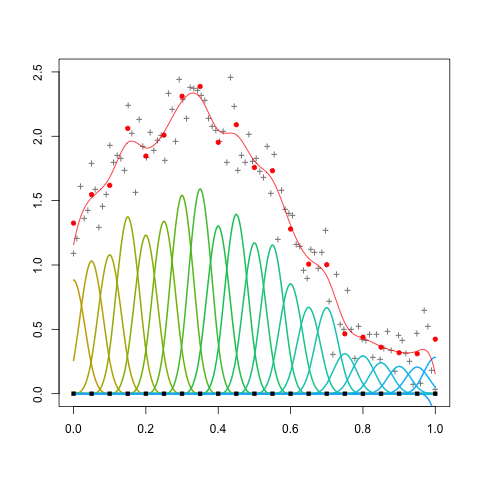
\includegraphics[scale=0.5]{pspline_pord2_xsmall_lambda.png}
  \label{fig:pspline_small_lambda}
\end{subfigure}
\begin{subfigure}{.5\textwidth}
  \centering
   \graphicspath{{img/}}
  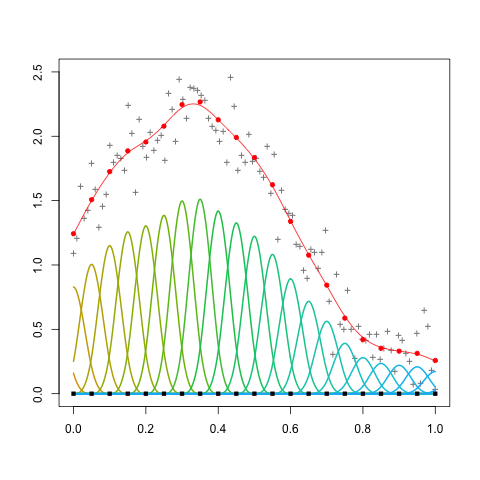
\includegraphics[scale=0.5]{pspline_pord2_small_lambda.png}
  \label{fig:pspline_small_lambda}
\end{subfigure}
\begin{subfigure}{.5\textwidth}
  \centering
   \graphicspath{{img/}}
  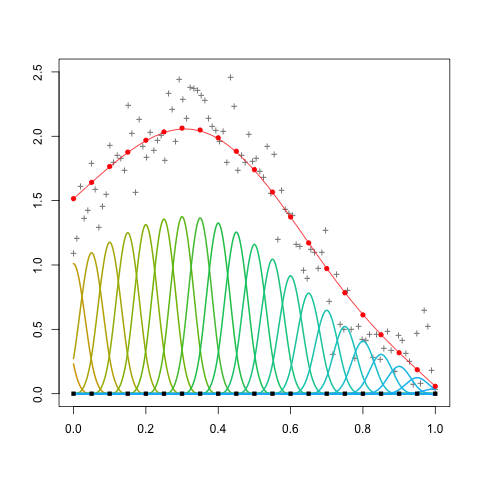
\includegraphics[scale=0.5]{pspline_pord2_medium_lambda.png}
  \label{fig:pspline_small_lambda}
\end{subfigure}
\begin{subfigure}{.5\textwidth}
  \centering
   \graphicspath{{img/}}
  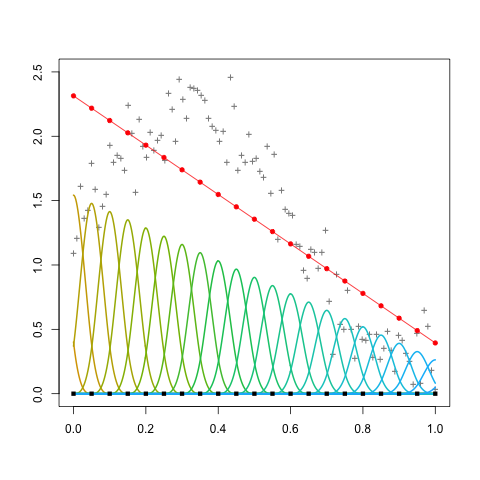
\includegraphics[scale=0.5]{pspline_pord2_large_lambda.png}
  \label{fig:pspline_small_lambda}
\end{subfigure}
\caption{\textit{Illustration of the impact of the second order difference penalty. The number of B-splines used is the same in each plot, with the value of the penalty parameter increasing from left to right and top to bottom across each plot. The fitted curve in the upper left plot is the most ``wiggly'' of any of the fits, as the penalty plays the weakest roll in the fitted coefficients there. The red circles are the values of each of the B-spline coefficients; as the penalty increases, they form as smoother sequence as we move across the four plots, which results in a smoother fitted function. As the penalty parameter approaches infinity, the fit approaches a linear function as shown in the bottom right plot.}}
\label{fig:second-ord-PS-pen-SML-lambda}
\end{figure}


The number of B-splines can be much larger than the number of observations because penalty ensures that the fitting procedure is well-conditioned. Figure~\ref{fig:overcomplete_basis_pspline} illustrates this utility of the penalty for simulated data; there are $m=10$ observations and $60$ cubic B-splines. This property of P-splines cannot be overly appreciated because it frees us from the concern of choosing the optimal set of knots. Unless computational constraints are of concern, which is possible with large models, it is prudent to use even more B-splines. Figure~\ref{fig:PS_penalty_section_figure_2} shows how the fitted function changes as the tuning parameter varies when the data are sparsely sampled. 

\begin{figure}[H]   \label{fig:overcomplete_basis_pspline}
  \centering
   \graphicspath{{img/}}
  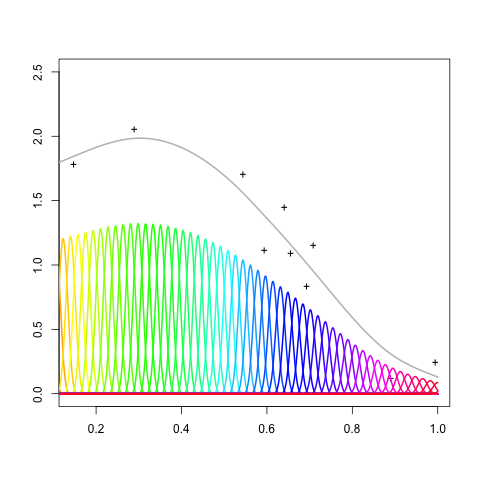
\includegraphics[scale=0.75]{pspline_10obs_60_basis_functions.png}
  \caption{P-spline smoothing of 10 observations using 60 B-spline basis functions.}
\end{figure}

\begin{figure}[H] \label{fig:PS_penalty_section_figure_2}
\centering
 \graphicspath{{img/}}
  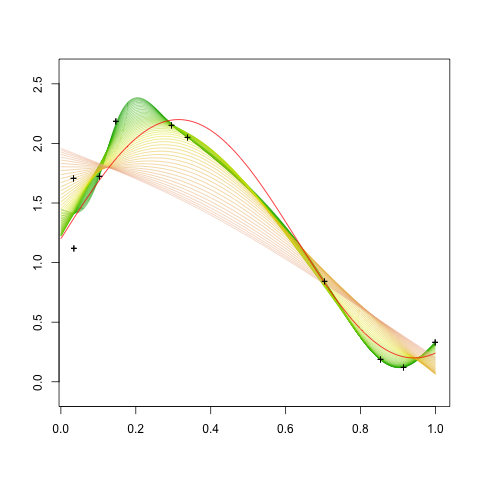
\includegraphics[width=4in, height=4in]{PS_penalty_section_figure_3.png}

  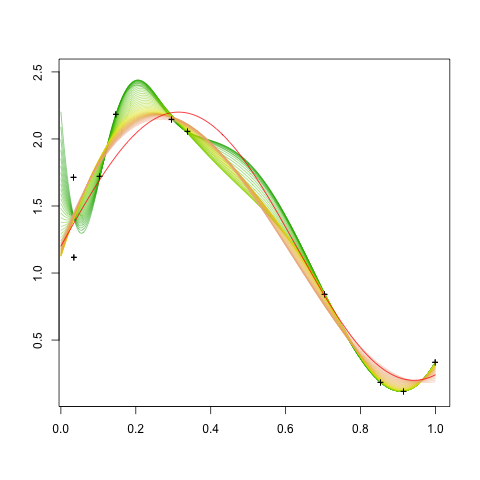
\includegraphics[width=4in, height=4in]{PS_penalty_section_figure_4.png}
 \caption{Fitted mean curves using a second (top) and third (bottom) order difference penalty for simulated data, sparsely sampled along the indexing variable: $y\left(t\right) = 1.2 + \sin\left(5t\right) + 0.2\epsilon_t$, where $\epsilon_t \stackrel{i.i.d.}{\sim}\textup{N}\left(0,1\right)$. A total of 10 data points were fit using a basis of 60 B-splines of degree $k=3$.}
\end{figure}

P-splines enjoy many advantageous properties, many of which are inherited from the attractive properties of B-splines. First, unlike many types of kernel smoothers, P-splines show no boundary effects i.e. the spreading of the fitted curve outside of the physical domain of the data, usually while also bending toward zero. See \citet{eilers1996flexible} Section 8 for a detailed discussion.

P-splines can fit polynomial data exactly. Given data $\left(l_i,y_i\right)$, if the $y_i$ are a polynomial in $l$ of degree $k$, then B-splines of degree $k$ or higher will fit the data exactly.  The same is true for P-splines if the order of the penalty is $k+1$ or higher, irrespective of the value of $\lambda$. An informal proof is left to the appendix.

Under a difference penalty of order $k$, the fitted function will approach a polynomial of degree $k-1$ for large values of $\lambda$ as long as the degree of the B-splines is greater than or equal to $k$. This can be shown by once again considering the relationship between the derivatives of a B-spline fit and the differences in neighboring coefficients; detailed discussion is left to the appendix. Figure~\ref{fig:PS_penalty_section_figure_6} visually demonstrates this property by examining the behavior of the fitted function as the tuning parameter varies under a difference penalty of order $d=0,1,2,3$.

We will leverage several properties of the smoothing matrix, $H$, for model evaluation and selection, so focus on the linearized smoothing problem solved at each value of the penalty parameter, $\lambda$, is prudent. The trace of $H$ approaches the order of the differencing operator, $k$ for larges values of $\lambda$. The trace of the smoothing matrix is a useful measure of effective model dimension, so understanding its limiting behavior is important. 



\begin{figure}[H]
\begin{subfigure}{.5\textwidth}
  \centering
   \graphicspath{{img/}}
  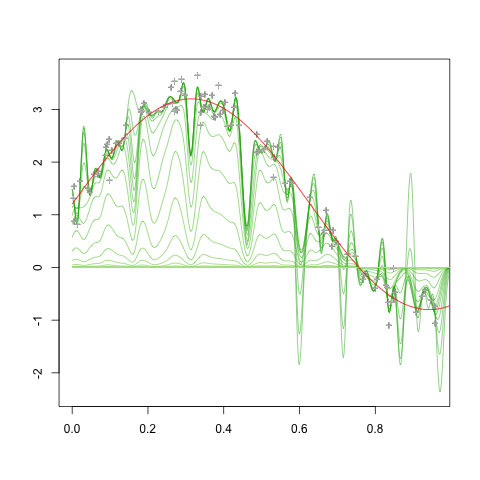
\includegraphics[scale=0.5]{PS_penalty_section_figure_6_order_0.png}
  %\label{fig:pspline_small_lambda}
\caption{$d=0$ }
\end{subfigure}
\begin{subfigure}{.5\textwidth}
  \centering
   \graphicspath{{img/}}
  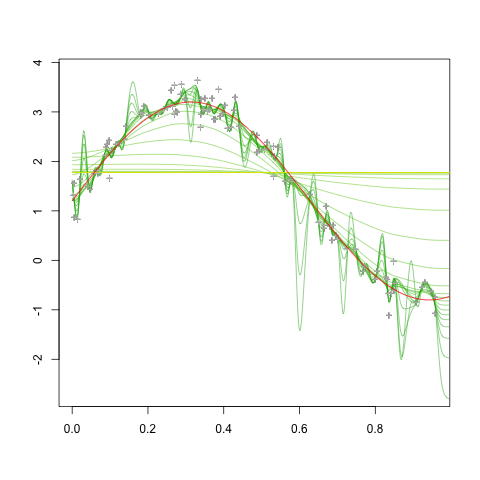
\includegraphics[scale=0.5]{PS_penalty_section_figure_6_order_1.png}
 % \label{fig:pspline_small_lambda}
\caption{$d=1$}
\end{subfigure}
\begin{subfigure}{.5\textwidth}
  \centering
   \graphicspath{{img/}}
  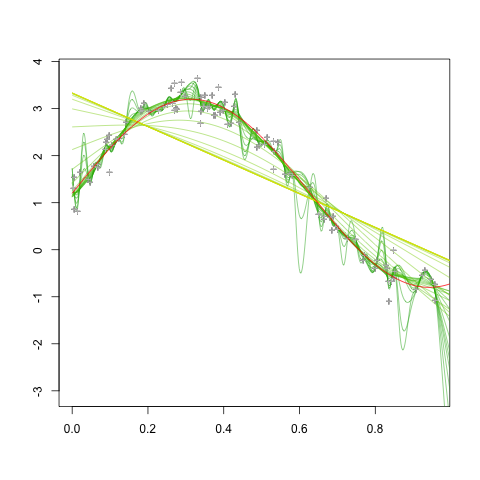
\includegraphics[scale=0.5]{PS_penalty_section_figure_6_order_2.png}
  %\label{fig:pspline_small_lambda}
\caption{$d=2$}
\end{subfigure}
\begin{subfigure}{.5\textwidth}
  \centering
   \graphicspath{{img/}}
  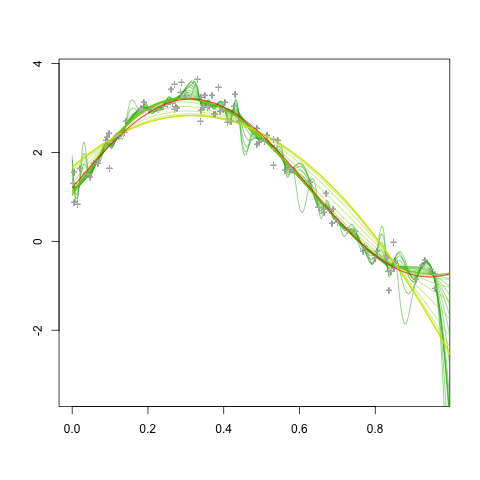
\includegraphics[scale=0.5]{PS_penalty_section_figure_6_order_3.png}
  %\label{fig:pspline_small_lambda}
\caption{$d=3$}
\end{subfigure}
\caption{\textit{Illustration of the impact of the order of the difference penalty. The number of B-splines used is the same in each plot, with the penalty parameter varying from across the same grid of values. The fitted curves in the upper left plot correspond to the difference penalty of order $0$, where $\vert D_0 \alpha \vert^2 = \sum_{i=1}^n \alpha_i^2$, analogous to ridge regression using the B-spline basis as regression covariates. The fitted curves approach polynomials of degree $d-1$ as $\lambda \rightarrow \infty$.}}
\label{fig:PS_penalty_section_figure_6}
\end{figure}


\subsection{Multidimensional smoothing with B-splines} \label{subsection:tensor-product-pspline-models}

P-splines can be extended naturally to higher dimensions by constructing a regression basis from the tensor product of the one-dimensional B-splines bases for each dimension. Figure~\ref{fig:bicubic_BS} displays the building block of the foundation on which multidimensional P-splines is built: a B-spline tensor product basis $\big\{ T_{kl}\big\}$ function.  If we equip $l$ and $m$ each with a B-spline basis, we can a basis for the varying coefficient function $\phi$ in \ref{eq:phi-star} by taking the tensor product of the two marginal bases. To regularize the fitted function, the only other modification necessary for the extension into two dimensions is the addition of a difference penalty for each variable $l$ and $m$. Let $B_{1}\left(l\right),\dots, B_{K}\left(l\right)  \mbox{ and } B_{1}\left(m\right),\dots, B_{L}\left(m\right)$  denote the B-spline bases for $l$ and $m$, each having a set of equally spaced knots along their respective domain. It is worth noting that while we have chosen not to distinguish between $\left\{ B_k \right\}$ and $\left\{ {B}_l \right\}$ for the sake of brevity, one is free to specify a different basis for each dimension either by using different order B-spline or, of course, using different numbers of knots, and hence entirely different knot sequences since P-splines rely on bases with equally spaced knots. The tensor product basis functions
\begin{equation*}
T_{jk}\left(l,m\right) = B_j\left(l\right){B}_k\left(m\right)
\end{equation*}
\noindent
 carve the $l$-$m$ domain into rectangles.  Figure~\ref{fig:sparse_bicubic_BS_basis} shows a thinned tensor product basis $\left\{ T_{kl} \right\}$l; a portion of the basis was omitted to eliminate overlapping of the basis functions so that the reader can identify individual tensor products. Each ``hill'' in Figure~\ref{fig:sparse_bicubic_BS_basis} is associated with an unknown coefficient $\alpha_{ij}$ which determines the height of the hill. For a given knot grid, we can approximate a surface by


\begin{equation} \label{eq:varying-coefficient-tensor-product-expansion}
\phi^*\left(l,m\right) = \sum_{i=1}^K \sum_{j=1}^L \alpha_{ij} B_{i}\left(l\right) B_{j}\left(m\right).
\end{equation}


\begin{figure}[H]
\centering
 \graphicspath{{img/}}
  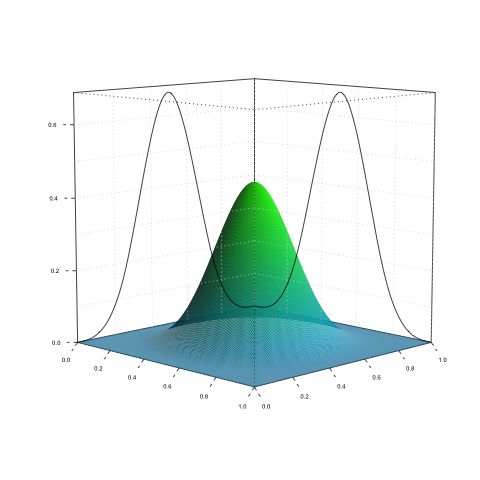
\includegraphics[width=4in, height=4in]{bicubic_basis_function.png}
 
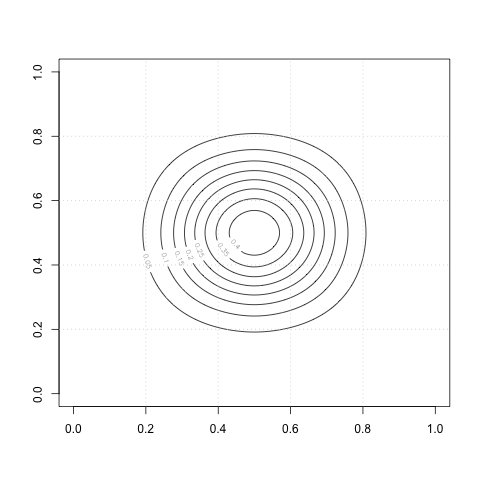
\includegraphics[width=4in, height=4in]{bicubic_bspline_contour.png}
\caption{Tensor product of two cubic B-splines}
\label{fig:bicubic_BS}
\end{figure}

\begin{figure}[H]
  \centering
  \graphicspath{{img/}}
  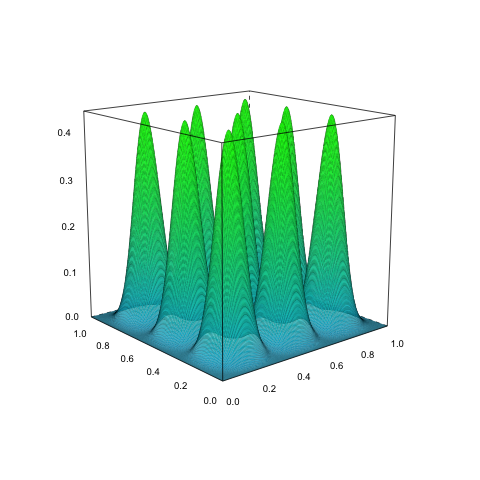
\includegraphics[width=5in,height=5in]{sparse_bicubic_basis.png}
  \caption{A subset of a full bivariate basis of cubic B-splines}\label{fig:sparse_bicubic_BS_basis}
\end{figure}



Let $p$ denote the total number of unique within-subject pairs of design points, and index the transformed coordinate pairs $\left( l,m \right)_i$, $i=1, \dots,p$. Let $B_l$ and $B_m$ denote the B-spline bases along the $l$ and $m$ coordinates of dimension $p \times K$ and $p \times L$, respectively, and let $A$ be the unknown matrix of basis coefficients with elements $\left[ \alpha_{ij} \right]$. To control the flexibility of the fitted function as with univariate P-splines discussed in Section~\ref{subsection:univariate-psplines}, we can apply difference penalties to the rows and columns of $A$ to smooth in the $l$ and $m$ directions respectively, using the penalty 

\begin{equation}\label{eq:unfolded-row-column-difference-penalty}
\lambda_l \sum_{k} \vert D_d \alpha_{k \cdot} \vert^2 + \lambda_m \sum_{l} \vert D_{\ms d_{\ms m}} \alpha_{\cdot l} \vert^2 .
\end{equation}
\noindent
where $\alpha_{k \cdot}$ and $\alpha_{\cdot l}$ denote the $k^{th}$ row and $l^{th}$ column of $A$, respectively. The first term in\ref{eq:unfolded-row-column-difference-penalty} imposes a difference penalty of order $d_{\ms l}$ on the rows of the coefficient matrix while the second term places a difference penalty (of possible different order $d_{\ms m}$) on the columns. We give each direction its own smoothing parameter to permit anisotropic smoothing; however, one could opt to use a single smoothing parameter for both directions and dodge the added work of optimizing the amount of smoothing with two separate parameters. Figure ~\ref{fig:2d_PS_penalty_demo} shows a potential result of heavy column penalization (left) and heavy row penalization (right) under a second order difference penalty on each row and each column for large values of $\lambda_l$ and $\lambda_m$. The figure demonstrates that the limiting behaviour of each row and column is linear, but the resulting surface may exhibit slope reversals from one row (column) to the next. 


\begin{figure}[H] \label{fig:2d_PS_penalty_demo}
 \begin{subfigure}{.48\textwidth}
  \centering
   \graphicspath{{img/}}
 \includegraphics[scale=0.5]{"model selection/effective dimension/2d_PS_section_figure1_big_col_lambda"}
 \caption{\textit{heavy column penalty}}
 \label{fig:2D_PS_big_col_penalty}
 \end{subfigure}
 \begin{subfigure}{.48\textwidth}
  \centering
   \graphicspath{{img/}}
  \includegraphics[scale=0.5]{"model selection/effective dimension/2d_PS_section_figure1_big_row_lambda"}
 \caption{\textit{heavy row penalty}}
\label{fig:2D_PS_big_row_penalty}
 \end{subfigure}
 \caption{\textit{Nine cubic B-spline tensor products with heavy linear column penalty and heavy linear row penalty}}
\end{figure}
\noindent
We take the estimator of $\phi^*$ to be the minimizer of 

\begin{align} 
\begin{split}\label{eq:unfolded-difference-penalty-log-likelihood}
-2L + J\left(\phi^*\right) = \sum_{i=1}^N \sum_{j=2}^{m_i} \sigma\left({t_j}\right)^{-2} \left\{y_{ij} - \sum_{k=1}^{j-1} \left( \sum_{r=1}^L \sum_{s=1}^K \alpha_{rs} B_r\left(l_{ijk}\right)B_s\left(m_{ijk}\right)\right)y_{ik} \right\}^2 \\ 
+ \lambda_l \sum_{r^\prime=1}^K \vert D_{d_{\ms l}} \alpha_{r^\prime \cdot} \vert^2 + \lambda_m \sum_{s^\prime=1}^L \vert D_{d_{\ms m}} \alpha_{\cdot s^\prime} \vert^2.
\end{split}
\end{align}

It is computationally advantageous to express the coefficient matrix in ``unfolded'' notation, which allows us to express the varying coefficient function at the observed coordinate grid as in the usual multiple regression form:

\begin{equation*}
\mbox{vec}\left\{\phi^*\left(l,m\right)\right\} = B \alpha
\end{equation*}
\noindent
Stacking the columns of $A$ gives the vectorized coefficient matrix $\alpha = \mbox{vec}\left( A \right)$. The $p \times KL$ tensor product basis $B$ is constructed from the tensor product of the marginal B-spline bases defined in \citet{eilers2006fast} as the \textit{row-wise Kronecker product} of the individual bases:

\begin{equation} \label{eq:rowwise-kronecker-product}
B = B_l \square B_m = \left( B_m \otimes 1^T_{K} \right) \odot \left(1^T_{L} \otimes  B_l  \right).
\end{equation}
\noindent
The operator $\odot$ denotes the element-wise matrix product; $1_K$ ($1_L$) denotes the column vector of ones having length $K$ ($L$.) The operations in \ref{eq:rowwise-kronecker-product} construct $B$ such that the $i^{th}$ row of $B_m\square B_l$ is the Kronecker product of the corresponding rows of $B_m$ and $B_l$. The penalty in \ref{eq:unfolded-row-column-difference-penalty} can also be compactly expressed:

\begin{equation} \label{eq:tensor-product-penalty}
\lambda_l \vert P_l \alpha \vert^2 + \lambda_m \vert P_m \alpha \vert^2
\end{equation}

where $P_l = I_L \otimes D_{d_{\ms l}}^T D_{d_{\ms l}} $ and $P_m =  D_{d_{\ms m}}^T D_{d_{\ms m}} \otimes I_K$. We define the matrix $W$ of historical regressors so that \ref{eq:unfolded-difference-penalty-log-likelihood} can be written in matrix form as

\begin{equation} \label{eq:tensor-pspline-objective-function}
-2L + J\left(\phi^*\right) = \vert Y - WB\alpha \vert^2 + \lambda_l \vert P_l \alpha \vert^2 + \lambda_m \vert P_m \alpha \vert^2,
\end{equation}
\noindent
with $\hat{\alpha}$ solving the system of equations 
\begin{equation} \label{eq:tensor-pspline-normal-equations}
\left[ \left(WB\right)^T WB +  \lambda_l P_l+ \lambda_m P_m\right]\alpha = W B Y
\end{equation}
\noindent
From \ref{eq:tensor-pspline-normal-equations}, we note that the system of equations depends on basis coefficients remains fixed at $KL$, even as the number of observations increases.   The grid of regression coefficients can be recovered by arranging the elements of $\hat{\alpha}$ into a matrix of $L$ columns having length $K$. The effective hat matrix is given by 
\[
H_\lambda = W B\left(W B^T W B +  \lambda_l P_l + \lambda_m P_m \right)^{-1} W B^T,
\]
from which we can easy calculate deletion residuals and obtain a measure of effective model dimension. We will discuss diagnostics and approaches to model selection in detail in Section~\ref{}.

\section{P-spline ANOVA models for $\phi^*$}

An extension of the tensor product models in \ref{subsection:tensor-product-pspline-models} for the varying coefficient function corresponding to the Cholesky factor $T$ is the class of multidimensional models like in Section~\ref{} based on the decomposition of multidimensional smooth functions as additive terms and interactions. Smoothing spline analysis-of-variance models have been previously proposed by \citet{gu1993semiparametric}, \citet{wahba1995smoothing}, and \citet{gu2002smoothing}, which gives main effects and interaction terms that can be interpreted as in the classical ANOVA setting. More recently, \citet{lee2011p} proposed the use of P-splines within a mixed modeling framework to estimate multidimensional functions as a decomposition into smooth main effects and interactions. They show that identifiability of functional components is ensured by imposing the same constraints as in a factorial design. 

As in the smoothing spline formulation, we may decompose
\begin{equation} \label{eq:SANOVA-model}
\phi^*\left(l,m\right) = \mu + \phi_1\left(l\right) + \phi_2\left(m\right) + \phi_{12}\left(l,m\right),
\end{equation} 

where $\mu$ is a constant, $\phi_1$ and $\phi_2$ are the additive univariate functions of $l$ and $m$, and $\phi_{12}$ is the two-dimensional interaction smooth function of $\left(l,m\right)$. The smooth-ANOVA model is given by

\begin{equation} \label{eq:SANOVA}
E\left[ Y \right] = W  B \theta
\end{equation}
\noindent
where $W$ is defined as in \ref{eq:tensor-pspline-objective-function}. The B-spline regression basis $B$ is defined 

\begin{equation} \label{eq:SANOVA-basis-matrix}
B = \left[\; 1_p \; \vert \;  B_l  \; \vert \;   B_m \; \vert B_{lm} \; \right]
\end{equation}
\noindent
where $B_{lm}$, the basis for the $l$-$m$ interaction term, is defined as in \ref{eq:rowwise-kronecker-product}. The full regression basis has dimension $p \times \left( 1 + K + L + KL \right)$; the vector of regression coefficients is given by $\theta = \left(\mu, \theta_l, \theta_m, \theta_{lm}\right)^T$, where $\theta_l$ and $\theta_m$ are the $K \times 1$ and $L \times 1$ vectors of coefficients for the main effects and $\theta_{lm}$ is the $KL \times 1$ vector of coefficients for the smooth $l$-$m$ interaction. The $\left(1 + K + L + KL\right) \times \left(1 + K + L + KL\right)$ penalty matrix is given by 

\begin{align}
\begin{split} \label{eq:PSANOVA-penalty}
P &= \mbox{blockdiag}\left\{0, P_l, P_m, P_{lm}\right\}\\ 
&= \begin{bmatrix}
0 	 & \dots 		      &    			 	& \\
\vdots &  \lambda_l D_{d_{\ms l}}^T D_{d_{\ms l}} &				 	& \\
&   	 			      &  \lambda_m D_{d_{\ms m}}^T D_{d_{\ms m}} 	& \\
&	 &			      &					&  \tau_l \left(I_L \otimes D_{d_{\ms l}}^T D_{d_{\ms l}}\right) + \tau_m \left(D_{d_{\ms m}}^T D_{d_{\ms m}} \otimes I_K \right)			
\end{bmatrix},
\end{split}
\end{align}
\noindent
with the one-dimensional penalties for each of the additive terms (with corresponding smoothing parameters $\lambda_l$ and $\lambda_m$) and the two-dimensional penalty (with two additional smoothing parameters $\tau_l$ and $\tau_m$) for the interaction term making up the blocks. $D_{d_{\ms l}}$ and $D_{d_{\ms m}}$ are the difference matrices of order $d_{\ms l}$ and $d_{\ms m}$ respectively. With the new basis and penalty, the penalized likelihood \ref{eq:tensor-pspline-objective-function} becomes

\begin{equation} \label{eq:PSANOVA-objective-function}
-2L + J\left(\phi^*\right) = \left( Y - WB\theta \right)^T\left( Y - WB\theta \right) +  \theta^T P \theta.
\end{equation}


The basis $B$, however, is not of full rank; some of the elements of $B_l$ and $B_m$ are also included in the interaction basis $B_{lm}$, so $1 + K+ L$ columns of $B$ are linearly dependent. This identifiability problem is also reflected in the rank deficiency of the penalty matrix; for penalty matrices $D_l^\prime D_l$ and $D_m^\prime D_m$ of order $d_{\ms l}$ and $d_{\ms m}$ respectively, 
\begin{align*}
\mbox{rank}\left(P\right) &=  \mbox{rank}\left(P_l\right) + \mbox{rank}\left(P_m\right) + \mbox{rank}\left(P_{lm}\right) \\
&= \left(K - d_{\ms l}\right) + \left( L - d_{\ms m}\right) +  \left(K - d_{\ms l}\right)\left( L - d_{\ms m}\right)
\end{align*}

Model \ref{eq:SANOVA} must be modified to remove this redundancy and ensure identifiability of functional components. \citet{wood2017generalized} (Chapter 4) proposed the use of the QR decomposition to identify linearly dependent columns of the regression basis numerically, and then removing them from the basis. Alternatively, \citet{lee2011p} proposed a mixed model framework that allows for efficient smoothing parameter estimation and mitigates identifiability issues when one imposes the same constraints as in factorial designs. Under the mixed model formulation , the smoothing parameter becomes a ratio of the residual variance and the variance of the random effects, so smoothing parameter selection becomes a matter of estimating  variance components. 

\subsection{Mixed model representation of  P-splines}

\subsubsection {Mixed effects models}

Linear mixed effects models are an extension of the linear regression model to include random effects; the connection between mixed models and smoothing splines has been thoroughly explored. See \citet{},\citet{}, and \citet{}, for example. The interest in this particular representation is because it allows for smoothing to be included in a large class of models. Additionally estimation and inference for mixed models is already well established, and the use of mixed model methodology and software well already well developed and widely adopted.

Applying the appropriate transformation to the regression basis $B$ and the penalty $P$ can ensure that the functional components of the smooth-ANOVA model \ref{eq:SANOVA} are identifiable. \citet{lee2011p} proposed such a transformation described by \citet{currie2002flexible} which reparameterizes the model basis so that the PS-ANOVA model and its corresponding penalty can be represented as a mixed model:

\begin{equation}  \label{eq:vc-mixed-effects-model}
Y = W\left(X \beta + Z \alpha\right) + e, \quad \alpha \sim \mathcal{N}\left(0,G \right),\;\; e\sim\mathcal{N}\left(0, D \right),
\end{equation} 
\noindent
where $X$ and $Z$ are the model matrices for the fixed and random effects. $G = \sigma_\alpha^2 \Lambda$ holds the variance components of the random effects, $\alpha$, where $\Lambda$ is some positive definite matrix. The mixed model representation decomposes the varying coefficient function into an unpenalized part $X \beta$ and penalized smooth term $Z \alpha.$ Under the assumption of normality and $i.i.d.$ errors, one can carry out estimation of $\beta$, $\alpha$ and the variance components by restricted maximum likelihood. See \citet{schall1991estimation} or  \citet{patterson1971recovery} for detailed discussion of estimation of random effects models.  We will show that there is a one-to-one mapping between the variance components of the mixed model and the smoothing parameters of the original penalty \ref{eq:PSANOVA-penalty}, so smoothing parameter selection is accomplished through the usual estimation procedure for the mixed model.

\subsubsection{Estimation of mixed effects models}

Under the assumption of normality, from model \ref{eq:vc-mixed-effects-model}, the marginal distribution of $Y$ is normal with mean $X\beta$ and covariance 

\begin{equation} \label{eq:mm-marginal-covariance}
Cov\left(Y\right) = V = D + WZ G Z^\prime W^\prime,
\end{equation}
\noindent
and the log-likelihood is given by
\begin{equation} \label{eq:mm-log-likelihood}
\mathcal{L} \left( \beta, \alpha, D , \sigma_\alpha^2 \right) = -\frac{1}{2} \log\vert V \vert - \frac{1}{2} \left( Y - WX\beta \right)^\prime V^{-1}\left( Y - WX\beta \right). 
\end{equation}
\noindent
Fixing $D$ and $\sigma_\alpha^2$, taking derivatives with respect to $\alpha$ and $\beta$ and setting equal to zero gives

\begin{align} \label{eq:mm-coefficient-mles}
\begin{split}
\hat{\beta} &= \left( X^\prime W^\prime V^{-1}WX \right)^{-1}X^\prime W^\prime V^{-1} Y \\
\hat{\alpha} &= G\left( W Z \right)^\prime V^{-1} \left( Y-WX\hat{\beta} \right).
\end{split}
\end{align}

The maximum likelihood estimates, however, are biased because they do not account for the degrees of freedom lost in the estimation of the fixed effects. To account for this bias, one may employ restricted maximum likelihood estimation for estimation of mixed effects models. See \citet{schall1991estimation} for a detailed overview. The restricted maximum likelihood estimates for the variance components can be obtained by maximizing the residual profile log-likelihood:

\begin{align}
\begin{split} \label{eq:mm-restricted-log-likelihood}
\mathcal{L}_r \left( D , \sigma_\alpha^2 \right) =  -\frac{1}{2} \log\vert V \vert  &-\frac{1}{2} \log\vert X^\prime W^\prime V WX \vert \\
 &- \frac{1}{2} Y^\prime \left( V^{-1} - V^{-1}WX \left(X^\prime W^\prime V^{-1}WX \right)X^\prime W^\prime V^{-1} \right) Y
\end{split}
\end{align}
\noindent
Computational efficiency can be improved by avoiding the direct calculation of the determinant and inverse of $V$, which is a Schur complement. Using the properties of the Schur complement, one can show that 

[THIS NEEDS CORRECTED]

\begin{align}
\begin{split}
\vert V \vert &=  \prod_{j=1}^m \sigma_j^2 \vert G \vert  \vert G^{-1} + Z^\prime W^\prime D^{-1}WZ \vert \\
V^{-1} &= D^{-1} \left( I - WZ\left( G + Z^\prime W^\prime D^{-1} W Z \right)^{-1} Z^\prime W^\prime D  \right) 
\end{split}
\end{align}
\noindent 
which involves inverting matrices having dimension which relies on the number of random effect coefficients rather than the number of observations. 


\subsubsection{Mixed model representation of P-splines}

To reparameterize \ref{eq:SANOVA-basis-matrix}, one can find an orthogonal transformation, $M$, such that

\begin{align}
\begin{split} \label{eq:PSANOVA-to-mm-mapping}
BM &= \left[\; X \; \vert \; Z \; \right], \mbox{ and}\\
M \theta &= X \beta + Z \alpha,
\end{split}
\end{align}
\noindent
and $\left[\; X \; \vert \; Z \; \right]$ has full rank; i.e.
\begin{align*}
B M M^T \theta &= \left[\; X \; \vert \; Z \; \right]M^T \theta \\
&= \left[\; X \; \vert \; Z \; \right] \mu
\end{align*}
\noindent
where $\mu = \left(\beta^T,\alpha^T\right)^T$. This transformation converts the penalty $\theta^T P \theta$ to the form

\begin{equation*}
\theta^T M^T P M \theta = \alpha^T F \alpha,
\end{equation*}
\noindent
for some block diagonal matrix $F$.  The transformation matrix $M$ is derived from the SVD of the penalty matrix \ref{eq:PSANOVA-penalty} by simultaneously diagonalizing $D_l^T D_l$ and $D_m^T D_m$; details are left to the appendix. After applying the transformation $M$ to the PSANOVA basis \ref{eq:PSANOVA-basis-matrix} according to \ref{eq:PSANOVA-to-mm-mapping}, the fixed effect and random effect model matrices for the main effects are given by 


\begin{align} 
\begin{split} \label{eq:PSANOVA-fixed-random-effect-matrices}
X &= \left[ \begin{array}{c|c|c|c|c|c|c|c|c} 1 & l  & \dots & l^{\ms d_{\ms l}-1}& m \dots & m^{\ms d_{\ms m}-1} & \dots &  l^{\ms d_{\ms l}-1} \square m^{\ms d_{\ms m}-1} \end{array} \right] \\
Z &= \left[ \begin{array}{c|c|c|c|c|c|c} m \square Z_l & \dots &  m^{\ms d_{\ms m}-1} \square Z_l & Z_m \square l & \dots & Z_m \square  l^{\ms d_{\ms l}-1} & Z_m \square Z_l \end{array} \right]
\end{split}
\end{align}
\noindent 
where the random effects $Z_l$ and $Z_m$ are constructed by projecting the marginal bases for $l$ and $m$ onto the non-null eigenvectors of the SVD of the marginal penalties $D_{\ms d_{\ms l}}^\prime D_{\ms d_{\ms l}}$ and $D_{\ms d_{\ms m}}^\prime D_{\ms d_{\ms m}}$. See the appendix for further discussion. 


\begin{align}
\begin{split} \label{eq:PSANOVA-mm-marginal-matrices}
\phi_1\left(l\right) &\equiv \left[ \begin{array}{c|c} X_l & Z_l \end{array} \right] 	= \left[ \begin{array}{c|c|c|c|c} 1_p & l   &\dots & l^{\ms d_{\ms l} -1}     & Z_l \end{array} \right], \mbox{ and} \\
\phi_2\left(m\right) &\equiv \left[ \begin{array}{c|c} X_m & Z_m \end{array} \right]  =\left[ \begin{array}{c|c|c|c|c} 1_p & m &\dots & m^{\ms d_{\ms m} \ms{- 1 }} & Z_m \end{array} \right].
\end{split}
\end{align}
\noindent
The mixed model matrix for the interaction term is given by 
 
\begin{align}
\begin{split}\label{eq:PSANOVA-mm-interaction-matrix}
\phi_{\ms 12}\left(l,m \right) &\equiv  \left[ \begin{array}{c|c|c|c} X_m\; \square \; X_l &  X_m\; \square \; Z_l  &  Z_m\; \square \; X_l  &  Z_m\; \square \; Z_l  \end{array} \right] \\
&\equiv 
\left[ 
\begin{array}{c|c|c|c}
 	\left[ \begin{array}{c|c} 1 & m \end{array} \right]  \square  \left[ \begin{array}{c|c} 1 & l \end{array} \right]& 
	\left[ \begin{array}{c|c} 1 & m \end{array} \right]  \square Z_l &
	 Z_m \square  \left[ \begin{array}{c|c} 1 & l \end{array} \right]  &
 	Z_m \square Z_l  
\end{array} 
\right]
\end{split}
\end{align}
This parameterization make it easy to identify the columns of \ref{eq:PSANOVA-mm-marginal-matrices} that are contained in \ref{eq:PSANOVA-mm-interaction-matrix}. After removing the column of 1s from the interaction matrix and one of the main effect matrices, the matrices corresponding to the fixed and random effects are given by 

\begin{align} 
\begin{split} \label{eq:PSANOVA-fixed-random-effect-matrices}
X &= \left[ \begin{array}{c|c|c|c|c|c|c|c|c} 1 & l  & \dots & l^{\ms d_{\ms l}-1}& m \dots & m^{\ms d_{\ms m}-1} & \dots &  l^{\ms d_{\ms l}-1} \square m^{\ms d_{\ms m}-1} \end{array} \right] \\
Z &= \left[ \begin{array}{c|c|c|c|c|c|c} m \square Z_l & \dots &  m^{\ms d_{\ms m}-1} \square Z_l & Z_m \square l & \dots & Z_m \square  l^{\ms d_{\ms l}-1} & Z_m \square Z_l \end{array} \right]
\end{split}
\end{align}

To obtain the variance-covariance matrix of the mixed model $G = \sigma_\epsilon^2 F^{-1}$, one may use the fact that $F = M^\prime P M$. The transformation matrix $M$ must take into account the reduced dimension of the mixed model matrices $X$ and $Z$. The resulting matrix is block diagonal, with a block for each of the functional components. 

\subsubsection{PSANOVA transformation matrix, $M$}

Removing the $1_p$ vector from the mixed model matrices is equivalent to removing the first column from the eigenvectors spanning the null space of each of the marginal penalties, $U_{l0}$ and $U_{m0}$, i.e. excluding $1_l^*$ and  $1_m^*$ from $M$. The $\left( 1 + K + L + KL \right) \times KL$ transformation matrix for the PS-ANOVA model is given by 

\begin{align}
\begin{split}
M &= \left[ \begin{array}{c|c}  M_0 & M_1  \end{array} \right] \\
&= \left[ \begin{array}{c|c}  M_0 & \begin{array}{c} 0 \\ M_1^* \end{array}  \end{array} \right] 
\end{split}
\end{align}
\noindent
where

\begin{align}
\begin{split} \label{eq:PSANOVA-transformation-matrix}
%M_0 &= \mbox{blkdiag}\left(1,  u_{\ms l1}^*, \dots,u_{\ms l,\ms d_{\ms l} \ms -1}^*,  u_{\ms m1}^*, \dots,u_{\ms m,\ms d_{\ms m} \ms -1}^*,  u_{\ms l1}^*  \otimes u_{\ms m1}^*, \dots,u_{\ms m,\ms d_{\ms m } \ms -1}^* \otimes u_{\ms l,\ms d_{\ms l } \ms -1}^*  \right), \\
M_0 &= \mbox{blkdiag}\left(1,  U^*_{ l0},  U^*_{ m0}, U^*_{ m0} \otimes  U^*_{ l0} \right), \\
M_1^* &= \mbox{blkdiag}\left( U_{l1}, U_{m1}, \bigg[ \begin{array}{c|c|c} U^*_{ m0} \otimes U_{l1}  & U_{m1} \otimes  U^*_{\ms l0}  &  U_{m1} \otimes  U_{ l1} \end{array} \bigg] \right) 
\end{split}
\end{align} 
\noindent 
where
\begin{align} 
\begin{split}\label{eq:marginal-difference-penalty-null-basis}
U_{l0} &= [\begin{array}{c|c} 1_K^* & U_{l0}^*  \end{array}] \\
&= [\begin{array}{c|c|c|c} 1_K^* & u_{\ms l1}^* & \dots & u_{\ms l,d_{\ms l}-1}^* \end{array}]
\end{split}
\end{align}
\noindent
is the $K \times d_l$ matrix corresponding to the null space of the $d_l^{th}$ order difference penalty, $D_{\ms d_{\ms l}}^\prime D_{\ms d_{\ms l}}$. Here,
\[
1_K^*= 1_K/\sqrt{K}
\]
denotes the $K$-vector of 1s scaled to have length 1, and the columns of $U_{l0}^*$ comprise a subset of orthogonal polynomials of degree $1,\dots, d_l-1$ centered around 0 so that 
\[
{u_{\ms li}^*}^\prime u_{\ms lj}^*  = \delta_{ij}.
\]
The submatrices $U_{l1}$ and $U_{m1}$ in \ref{eq:PSANOVA-transformation-matrix} are derived from the non-null eigenvectors of the $d_l^{th}$ and $d_m^{th}$ order difference penalties, as in the definition of \ref{eq:tensor-product-transformation-matrix}. Applying the transformation to $P$, the penalty becomes

\begin{equation} \label{eq:PSANOVA-mm-penalty}
F = \mbox{blkdiag}\left( 0, F_l, F_m, F_{lm}  \right) 
\end{equation}
\noindent
where
\begin{align*}
\begin{split} 
F_l &= \lambda_l \tilde{\Delta}_l,\\
F_{\ms m} &= \lambda_m \tilde{\Delta}_m, \mbox{ and}\\
F_{\ms l \ms m} &= \mbox{blkdiag}\left( \tau_l \tilde{\Delta}_l, \tau_l \tilde{\Delta}_l, [ \tau_l I_{L-d_{\ms m}} \otimes \tilde{\Delta}_l ]+ [ \tau_m \tilde{\Delta}_m \otimes I_{K-d_{\ms l}}] \right).
\end{split}
\end{align*}

\citet{lee2011p} showed that removing the column of $1$s from the fixed effect matrices for each of the marginal components \ref{eq:PSANOVA-mm-marginal-matrices} is equivalent to  imposing the same constraints on model coefficients as in the usual factorial design model. To see this, consider the recovered penalty of the original parameterization:

\begin{equation}\label{eq:recovered-penalty-matrix}
\tilde{P} = MFM^\prime = MM^\prime P M M^\prime
\end{equation}
where $P$ and $F$ are defined as in \ref{eq:PSANOVA-penalty} and \ref{eq:PSANOVA-mm-penalty}, respectively. However, $M$ is not orthogonal for the PSANOVA model with basis \ref{eq:SANOVA-basis-matrix}. One can show that $\mathscr{K} = M M^\prime$ is a centering operator:

\begin{equation} \label{eq:PSANOVA-centering-matrix}
\mathscr{K} = \begin{bmatrix}
1 	&    \dots	&	& 0 \\
 \vdots	&    \mathscr{K}_l	&	&\\
	& 	& \mathscr{K}_m	& \\
0 & & & \mathscr{K}_m \otimes \mathscr{K}_l
\end{bmatrix}
\end{equation}
\noindent 
where $\mathscr{K}_l = I_K - 11^\prime/K$ and $\mathscr{K}_m = I_L - 11^\prime/L$. See Appendix~\ref{subsection:transformation-centering-matrix-equivalence} for a detailed proof. The recovered penalty can be rewritten from \ref{eq:recovered-penalty-matrix} as

\begin{equation} \label{eq:recovered-PSANOVA-penalty}
\tilde{P} = \mathscr{K} P \mathscr{K},
\end{equation}
\noindent
with rank [DOUBLE CHECK THIS GENERALIZATION] $KL -  d_{\ms l} d_{\ms m}$. Applying the transformation to the coefficient vector $\theta$ in terms of $\mathscr{K}$ gives

\[
\theta^\prime \tilde{P} \theta = \tilde{\theta}^\prime P \tilde{\theta},
\]
where

\begin{equation} \label{eq:mm-parameter-constraints}
\tilde{\theta} \equiv \mathrm{K} \theta = \begin{bmatrix}\mu & \dots &  & \\
\vdots & \mathscr{K}_l  & &  \\
&&\mathscr{K}_m & \\
&&& \mathscr{K}_{m} \otimes \mathscr{K}_l 
\end{bmatrix} 
\begin{bmatrix} \mu \\ \theta_l \\ \theta_m \\ \theta_{lm} 
\end{bmatrix} \equiv \begin{bmatrix} \mu, \tilde{\theta}_l, \tilde{\theta}_m, \tilde{\theta}_{lm}  \end{bmatrix}^\prime
\end{equation}
\noindent
with
\begin{align}
\begin{split} \label{eq:main-effect-coefficient-constraints}
\tilde{\theta}_l = \mathscr{K}_l \theta_l, \\
\tilde{\theta}_m = \mathscr{K}_m \theta_m, \mbox{ and} \end{split} \\
\tilde{\theta}_{lm} = \mathscr{K}_{m} \otimes \mathscr{K}_l \theta_{lm} \label{eq:interaction-coefficient-constraint}
\end{align}
\noindent
The transformations in \ref{eq:main-effect-coefficient-constraints} center the coefficients corresponding to the main effects of $l$ and $m$, $\phi_1$ and $\phi_2$. If we write the right hand side of \ref{eq:interaction-coefficient-constraint} in array form, we have 
\[
\tilde{\Theta}_{lm} = \mathscr{K}_{l} \Theta_{lm}\mathscr{K}_{m},  
\]
which is equivalent to centering the coefficient matrix $\Theta_{lm}$ by rows and by columns. The transformation to the mixed model formulation enforces the same constraints on coefficients as those applied in a factorial design with two main effects and a 2-way interaction:

\begin{align}
\begin{split}
\sum_{i=1}^K \tilde{\theta}_{li} = \sum_{j=1}^L \tilde{\theta}_{mj} = 0, \mbox{ and}\\
\sum_{i=1}^K \tilde{\Theta}_{ij} = \sum_{j=1}^L \tilde{\Theta}_{ij} = 0.
\end{split}
\end{align}


\subsection{Restricted maximum likelihood estimation}

The previous section establishes the relationship between the variance components of the random effects in the mixed effects model \ref{eq:vc-mixed-effects-model}
















\section{Appendix} \label{appendix:appendix}


Proof of Theorem~\ref{phi_representer_thm}
 For simplicity of presentation, relabel the elements of $\mathcal{W}^*$ so that 
\[
\mathcal{W}^* = \lbrace \left( l_1,m_1 \right), \left( l_2,m_2 \right), \dots, \left( l_{N_{\phi^*}},m_{N_{\phi^*}} \right)  \rbrace.
\]
Then we may verify that any $\phi^* \in \mathcal{H}$ can be written 
\[
\phi^*\left(l,m \right) = d_0 + d_1k_1\left(l\right) + \sum_{i=1}^n  c_i R_1\left( \left(l,m\right) , \left(l_i,m_i \right)\right) + \rho\left(l,m\right)
\]
\noindent
where $\rho \perp \mathcal{H}_0 = \lbrace 1\rbrace \oplus \lbrace k_1\rbrace,\; span\lbrace R_1\left(\left(l_i, m_i \right),\cdot \right)  \rbrace$. We do so by demonstrating that  $\rho$ does not improve the first term in \eqref{eq:objectivefun} (the data fit functional) and only adds to the penalty term, $J\left(\phi^*\right)$. Consequently, if $\hat{\phi^*}$ is the minimizer of \eqref{eq:objectivefun}, then $\rho = 0$. Using the properties of reproducing kernels, we can rewrite $\phi^*$ as an inner product of itself with $R$:
 
\begin{eqnarray*}
\phi^*\left(l_j,m_j \right)  &=& \left< R\left(\left(l_j,m_j\right),\left(\cdot,\cdot\right) \right),\phi^*\left(\cdot,\cdot\right)\right>\\
&=& \left<R_0\left( \left(l_j,m_j\right),\left(\cdot,\cdot\right) \right) + R_1\left(\left(l_j,m_j\right),\left(\cdot,\cdot\right) \right),d_0 + d_1k_1\left(\cdot \right)\right. \\ 
&\mbox{ }&\left. \;\;\;\;\;\;\;\;\;\;\;\;\;\;\;\;\;\;\;\;\;\;\;\;\;\;\;\;\;\;\;\;\;+ \sum_{i=1}^{N_{\phi^*}}  c_i R_1\left( \left(l_i,m_i \right),\left(\cdot,\cdot\right) \right) + \rho\left(\left(\cdot,\cdot \right)\right)\right>\\
&=& \left<R_0\left( \left(l_j,m_j\right),\left(\cdot,\cdot\right) \right) , d_0 + d_1k_1\left(\cdot\right)\right> + \left< R_0\left( \left(l_j,m_j\right),\left(\cdot,\cdot\right) \right),\sum_{i=1}^{N_{\phi^*}}  c_i R_1\left( \left(l_i,m_i \right),\left(\cdot,\cdot\right) \right)\right> \\
&\mbox{ }& + \left<R_0\left( \left(l_j,m_j\right),\left(\cdot,\cdot\right) \right), \rho\left(\left(\cdot,\cdot \right)\right)\right> + \left<R_1\left(\left(l_j,m_j\right),\left(\cdot,\cdot\right) \right), d_0 + d_1k_1\left(\cdot \right)\right> \\
&\mbox{ }& + \left<R_1\left(\left(l_j,m_j\right),\left(\cdot,\cdot\right) \right),\sum_{i=1}^{N_{\phi^*}}  c_i R_1\left( \left(l_i,m_i \right),\left(\cdot,\cdot\right) \right) \right> + \left<R_1\left(\left(l_j,m_j\right),\left(\cdot,\cdot\right) \right), \rho\left(\left(\cdot,\cdot \right)\right)\right>\\
&=& \left<R_0\left( \left(l_j,m_j\right),\left(\cdot,\cdot\right) \right) , d_0 + d_1k_1\left(\cdot\right)\right> + \left<R_1\left(\left(l_j,m_j\right),\left(\cdot,\cdot\right) \right),\sum_{i=1}^{N_{\phi^*}}  c_i R_1\left( \left(l_i,m_i \right),\left(\cdot,\cdot\right) \right) \right> \\
&\mbox{ }& + \underbrace{\left<R_0\left( \left(l_j,m_j\right),\left(\cdot,\cdot\right) \right)  , \rho\left(\cdot,\cdot\right) \right>}_{0} + \underbrace{\left<R_1\left( \left(l_j,m_j\right),\left(\cdot,\cdot\right) \right)  , \rho\left(\cdot,\cdot\right) \right>}_{0}\\
&=& d_0 + d_1k_1\left(\cdot \right) + \sum_{i=1}^{N_{\phi^*}}  c_i R_1\left( \left(l_i,m_i \right),\left(l_j,m_j\right) \right)
\end{eqnarray*}
\noindent


Rewriting the data fit functional, we have that  
 \begin{eqnarray*}
&\mbox{ }&\sum_{i=1}^N \sum_{j=1}^{n_i} \sigma_{ij}^{-2} \left(y\left(t_{ij}\right) - \sum_{k=1}^{j-1} \phi^*\left(t_{ij}, t_{ik}  \right) y\left(t_{ik}\right)  \right)^2  \\ 
&=& \sum_{i=1}^N \sum_{j=1}^{n_i} \sigma_{ij}^{-2} \left(y\left(t_{ij}\right) - \sum_{k=1}^{j-1} \left< R\left(\left(l^i_{jk},m^i_{jk}\right),\left(\cdot,\cdot\right) \right),\phi^*\left(\cdot,\cdot\right)\right> y\left(t_{ik}\right)  \right)^2  \\
 \end{eqnarray*}
\noindent
which is free of $\rho$. Consider the contribution of any nonzero $\rho$ to $J\left(\phi^*\right)$: 
  
 \begin{eqnarray*}
 J\left(\phi^*\right) &=& \vert \vert  P_1\phi^* \vert \vert^2\\
 &=& \left< \sum_{i=1}^{N_{\phi^*}}  c_i R_1\left( \left(l_i,m_i\right),\left(\cdot,\cdot\right) \right) + \rho\left(\cdot,\cdot \right), \sum_{j=1}^{N_{\phi^*}} c_j R_1\left( \left(l_j,m_j\right),\left(\cdot,\cdot\right) \right) + \rho\left(\cdot,\cdot\right)\right> \\
 &=& \vert \vert \sum_{i=1}^{N_{\phi^*}}  c_i R_1\left(\left(l_i,m_i\right),\left(\cdot,\cdot\right) \right) \vert \vert^2 + \vert \vert  \rho \vert \vert^2 
 \end{eqnarray*}
\noindent
Thus, including $\rho$ in $\phi^*$ only increases the penalty without improving (decreasing) the data fit functional, so we indeed have that the minimizer of \eqref{eq:objectivefun} has the form
\begin{equation}
 \phi^*\left(l,m\right) =  d_0 + d_1k_1\left(l\right) + \sum_{i=1}^{N_{\phi^*}} c_i R_1\left( \left(l,m\right) , \left(l_i,m_i \right)\right)
 \label{eq:finitedimsolution}
 \end{equation}


Proof: Proposition~\ref{prop:cholesky-inverse-banding-equivalence}

\underline{\bf Proof:} Using the expression
\[
\sigma^{ij} = \sum_{k=i}^p d_{ii}t_{ki}t_{kj}
\]
it follows immediately that $t_{pj} = \dots = t_{r\left(j\right),j} = 0$ implies that $\sigma^{pj} = \dots = \sigma^{r\left(j\right),j} = 0$.

From cite{watkins2004fundamentals}, we can show that we can sequentially derive the elements of $T$ and $D$ according to 

\begin{eqnarray*}
d_{ii} = \sqrt{\sigma^{ii}-\sum_{k=1}^{i-1} t_{ki}^2 }\\
t_{ij} = \frac{1}{d_{ii}}\left(\sigma^{ij} - \sum_{k=1}^{i-1} t_{ki}t_{kj} \right)
\end{eqnarray*}
\noindent

We proceed by induction. For the first row of $T^T$, 

\subsection{Construction of the mixed model transformation matrix, $M$}

Let
\[
U_l \Delta_l U_l^T
\]
denote the singular value decomposition of $D_l^T D_l$, where $U_l$ is the $K \times K$ matrix of eigenvectors and $\Delta_l$ is the diagonal matrix with diagonal entries equal to the corresponding eigenvalues. Exactly $d_{\ms l}$ of of the eigenvalues are identically zero, so if we let $\tilde{\Delta}_l$ denote the submatrix containing only the positive eigenvalues, then we can write

\[
\Delta_l = \mbox{diag}\left( 0_{d_{\ms l}},\tilde{\Delta}_l \right).
\] 

Let 
\[
U_{l0} = \begin{bmatrix} 1_l^* & u_{l1}^* ... & u_{l,d_{\ms l} \ms - 1}^* \end{bmatrix}
\]
denote the matrix of eigenvectors corresponding to the zero eigenvalues, where $1_l^* = \left(1, 1, \dots,1 \right)^T/\sqrt{K}$ and $u_{li}^*$  is the vector having elements $\left( 1^i, 2^i,\dots,K^i \right)^T$, centered and scaled to have mean $0$ and unit length. Let $U_{l1}$ denote the submatrix of eigenvectors corresponding to the nonzero eigenvalues, $\tilde{\Delta}_l$. Define $U_{m0}$, $U_{m1}$, and $\tilde{\Delta}_{m}$ in the same fashion. 

The orthogonal transformation matrix $M$ is defined $M = \left[\begin{array}{c|c} M_0 & M_1 \end{array}\right]$, where

\begin{align} 
\begin{split} \label{eq:tensor-product-transformation-matrix}
M_0 &= \left[ \begin{array}{c} U_{m0} \otimes U_{l0} \end{array} \right], \mbox{ and} \\
M_1 &= \left[ \begin{array}{c|c|c}  U_{m0} \otimes U_{l1}  &  U_{m1} \otimes U_{l0}  &  U_{m1} \otimes U_{l1} \end{array} \right].
\end{split}
\end{align}

The transformed coefficients are given by 
\begin{equation*}
\beta = M_0^T\theta, \qquad \alpha = M_1^T\theta
\end{equation*}

Using properties of the kronecker product (see \citet{liu1999matrix}), one can show that the mixed model design matrices $X$ and $Z$ can be written as the tensor product of the marginal bases:

\begin{align}
\begin{split} \label{eq:mixed-model-tensor-matrices}
X &= \left[ \begin{array}{c} X_m \square X_l \end{array} \right], \mbox{ and} \\
Z &= \left[ \begin{array}{c|c|c} X_m \square Z_l & Z_m \square X_l & Z_m \square Z_l \end{array} \right].
\end{split}
\end{align}
\noindent
where 
\begin{align*}
X_l &= B_l U_{l0}, & &Z_l = B_l U_{l1}, \\ 
X_m &= B_m U_{m0}, & &Z_m = B_m U_{m1}.
\end{align*}
\noindent
This is convenient because the calculation of $M$ can be avoided in practice. Since $\beta$ is not penalized, we can replace $X_l$ and $X_m$ with 
\begin{equation*}
\left[\begin{array}{c|c|c|c} 1_p & l & \dots & l^{d_{\ms l} -1}  \end{array} \right] \mbox{ and } \left[\begin{array}{c|c|c|c} 1_p & m & \dots & m^{d_{\ms m} -1}  \end{array} \right]
\end{equation*}
Making this replacement, the expressions for $X$ and $Z$ can be expanded:
\begin{align}
X &= \left[ \begin{array}{c|c|c|c|c|c} 1_p & l & m & l \square m & \dots  & l^{\ms d_{\ms l} -1 } \square  m^{\ms d_{\ms m} -1 } \end{array} \right], \\
Z &= \left[ \begin{array}{c|c|c|c|c|c|c}  Z_l & Z_m & Z_m \square l & m \square Z_1 & \dots & Z_m \square l^{\ms d_{\ms l} \ms -1} & m^{d_{\ms m} -1} \square Z_1   \end{array} \right],
\end{align}
Construction of the fixed effects and mixed effects in this way allows us to express the fitted varying coefficient function $\phi^*$ as a sum of the main effects and an $l$-$m$ interaction. After applying the transformation, the penalty becomes

\begin{equation}
F = \begin{bmatrix}
0 	&	&	 & \\
	&  \lambda_l I_L \otimes \tilde{\Delta}_l  &	& \\
	&						& \lambda_m  \tilde{\Delta}_m\otimes & \\ 
&&&  \lambda_m  \tilde{\Delta}_m\otimes + \lambda_l I_L \otimes \tilde{\Delta}_l 
\end{bmatrix},
\end{equation} 
\noindent
where the $0$ element of the block diagonal is a matrix of zeros corresponding to the unpenalized fixed effects. The variance components of the mixed model are given by $G = \sigma_\epsilon^2 F^{-1}$. Applying these results to the smooth-ANOVA model \ref{eq:SANOVA} with regression basis \ref{eq:SANOVA-basis-matrix}, the mixed model matrices are given by 


\subsection{Transformation matrix $M$ imposes identifiability constraints} \label{subsection:transformation-centering-matrix-equivalence}

We can decompose the identity matrix according to 
\[
I = U_{l0}U_{l0}^\prime + U_{l1}U_{l1}^\prime
\]
where $U_{l0}U_{l0}^\prime = 1_K^* 1_K^{*\prime} + U_{l0}^*{U_{l0}^*}^\prime$. Then 

\begin{equation*} 
U_{l1}U_{l1}^\prime = I - 1_K^* 1_K^{*\prime} -  U_{l0}^*{U_{l0}^*}^\prime,
\end{equation*}
\noindent
where $1_K^* 1_K^{*\prime} = 1_K 1_K^{\prime}/K$. This gives
\begin{equation} \label{eq:appendix-transformation-proof-1} 
U_{l1}U_{l1}^\prime +  U_{l0}^*{U_{l0}^*}^\prime= I_K - 1_K^* 1_K^{*\prime}.
\end{equation}
After substituting \ref{eq:appendix-transformation-proof-1} into the definition of $M$ \ref{eq:PSANOVA-transformation-matrix}, it follows immediately that $MM^\prime = \mathscr{K}$ as it is defined in \ref{eq:PSANOVA-centering-matrix}.

\bibliography{Master}
\end{document}
